%!TEX root = ../main.tex
%******************************
%	 Introduction 
%*****************************

\chapter{Introduction}  

\graphicspath{Figures/}

\begin{Abstract}
The intrinsic stochasticity of biochemical reactions introduces phenotypic heterogeneity in seemingly homogeneous populations of cells. This phenomenon has been widely studied in prokaryotic and eukaryotic systems and the functional role of phenotypic variation in development, health and disease is subject of ongoing research. Biological noise, a term to describe molecular variability between individual cells, arises from different sources in homogeneous cell populations. Intrinsic noise summarizes stochastic differences in transcription and translation between individual genes \citep{Elowitz2002, Raser2004, Sanchez2013}. Extrinsic noise on the other hand arises when cells are in different cellular states (e.g.~cell cycle, cell-to-cell signalling and metabolism)  \citep{Zopf2013, Iwamoto2016, Kiviet2014}. Recent technological advances allow the in depth analysis of biological noise in cell populations. Imaging methodologies \citep{Moffitt2016a} and single-cell “omics” techniques \citep{Bock2016} permit the quantification of thousands of mRNA species, the genomic sequence, its epigenetic modification, and selected sets of proteins per cell. Moreover, the development of multi-omics technologies introduced the possibility to link cell-to-cell variation between multiple regulatory layers across individual cells \citep{Macaulay2017}. With the emergence of single-cell RNA sequencing (scRNA-Seq) technologies, new computational strategies to quantify noise were introduced \cite{Brennecke2013, Vallejos2015, Kolodziejczyk2015cell, Buettner2015, Fan2015, Richard2016}. Applying high-throughput scRNA-Seq to mammalian systems characterised the functional role of biological noise in healthy as well as diseased contexts. Studies of recent years described changes in noise levels at different stages during embryonic development which hints at stochastic contributions to early cell fate decisions \citep{Goolam2016, Mohammed2017, Ohnishi2014}. Phenotypic variation in immune cells, possibly derived by transcriptional noise, increases cellular plasticity and facilitates the population response to pathogens \citep{Shalek2014, Kellogg2015a}. Conversely, genetic and non-genetic heterogeneity within cell populations was described as driver for cancer development \citep{Marusyk2012} and noise increases with age \citep{Martinez-jimenez2017, Enge2017}. Here, I introduce noise as an inherent feature of biological system and discuss its positive and negative consequences in cell populations. Furthermore, I outline recent developments of single-cell sequencing and imaging technologies and comment on robust ways of quantifying biological noise. Finally, I will summarise Bayesian inference as a powerful statistical framework to model transcriptional noise from scRNA-Seq data.
\end{Abstract}

\newpage

% Include different main sections of the introduction
Kello%!TEX root = ../intro.tex
%******************************
%	 Biological noise 
%*****************************

\section{Biology of expression noise} 

\cor{The intrinsic stochasticity of biochemical reactions contributes to a wide distribution of \glspl{mRNA} and proteins across a seemingly homogeneous populations of cells\citep{Elowitz2002}. 
In the scientific litearature, this phenomenon is referred to as “biological noise” (see \textbf{Box 1})}
All cellular systems are exposed to varying levels of noise and employ strategies to make use of or cope with this source of variation. 
The sources and consequences of biological noise have been studied in an array of viral, prokaryotic and eukaryotic systems \citep{Raj2010, Balazsi2011, Eldar2010}. 
Across these systems the extent of its function remains unclear. 

\begin{Comment}
\hspace{-2.5mm}\textbf{Box 1: Defining biological noise}\label{box1}\\
\small
Biological noise in cell populations \cor{is defined as} stochastic effects on transcription and translation that propagates to form cell-to-cell phenotypic differences. 
To \cor{understand} noise, one needs to distinguish between different sources of cell-to-cell variability in multiple measurable factors. 
On the broadest level, differences between single cells in a population can arise from structured and unstructured sources. 
When capturing cell populations that contain discrete cell states and/or cell types \citep{Paul2015, Ibarra-Soria2018, Rosenberg2018}, measuring cell-specific features results in the detection of non-stochastic but rather correlated (structured) differences between individual cells. 
When the cell population structure is not driven by correlated features (unstructured variation), continuous processes (e.g.~differentiation) can be the dominating source of cell-to-cell phenotypic variability \citep{Dahlin2018}. 
Computational approaches allow the detection of these trajectories (e.g.~via \gls{PCA} or pseudotime inference \citep{Trapnell2014, Angerer2015}). 
Therefore, \cor{my work and work of others \citep{Faure2017, Morgan2018} focus on studying "molecular phenotypic variability", independent of measurement errors, in homogeneous cell populations as proxy for biological noise}. \\

\cor{Classically and specifically in populations of bacteria} \citep{Elowitz2002}, biological noise has broadly been classified into intrinsic and extrinsic noise. 
Intrinsic noise originates from stochastic biochemical effects that directly influence mRNA and protein expression gene-specifically (e.g.~\gls{TF} binding dynamics, see \citep{Swain2002}). 
Extrinsic noise on the other hand introduces co-variation across multiple genes (also in a pathway specific manner \citep{Raser2005}) due to \cor{variations} in cell-specific factors such as stress response, mitochondrial maintenance, amino-acid synthesis \citep{Stewart-Ornstein2012} or cell cycle \citep{Zopf2013}. 
\cor{Within a population of bacteria,} intrinsic noise can therefore be measured as expression differences between co-regulated genes in one cell, while extrinsic noise is measured as co-regulated variance in gene sets across all cells.
\cor{In multicellular systems however, the observed molecular phenotypic variability is a combination of stochastic (noise) and deterministic effects, which are difficult to delineate.}
\end{Comment}

\newpage

It is crucial to differentiate between unicellular systems (prokaryotes, viruses, and yeast) in which biological noise supports responses to environmental changes and higher, multicellular eukaryotic systems where biological noise either benefits or obstructs cellular function depending on the tissue type and health state. 
\cor{Furthermore, measuring the stochastic component of biological noise is difficult and requires time-resolved reporter gene read-outs in truly homogeneous cell populations\citep{Elowitz2002}. 
Due to this, the majority of studies presented in this chapter use the observable molecular phenotypic variation in form of single-cell transcriptomic or proteomic read-outs as proxy for biological noise (see \textbf{Box 1}). 
This variation is confounded by unobserved deterministic processes (e.g subtle cell cycle variation) and delineating the stochastic and deterministic component is challenging.}

\subsection{Bet-hedging in unicellular systems}

Biological noise has been \cor{proposed} to trigger the differential decision between latency and replication in viruses such as \gls{HIV} and the $\lambda$-phage. 
In the case of the $\lambda$-phage, infected cells either reside in a lysogenic state where the genetic material of the virus is transmitted to daughter cells without inducing cell death, or a lytic state where the virus destroys the host cell \textbf{(Fig.~\ref{fig0:bedhedging})} \citep{Lieb1953}. 
Previous studies have shown that the lysis-lysogeny switch in $\lambda$-phage is driven by intrinsic and extrinsic noise \citep{Arkin1998, St-Pierre2008}. 
This idea has been extended by Zeng \textit{el al.}, 2010 where the lysis-lysogeny switch does not depend on a single noise-driven decision but on the sum of all individual phages per cell \citep{Zeng2010}. 
\cor{This results contradicts the earlier studies, which either modelled the decision event on the level of each phage or connected the decision event with cellular volume. 
In general, by summing across stochastic events or if one is able to predict the lysis-lysogeny decision based on cellular volume, the switch does not occur as stochastically as initially anticipated.}
In the case of \Gls{HIV}, the virus either rapidly replicates or resides in a long-lived latent state from which the virus can switch to replication \citep{Weinberger2015}. 
It has been shown that combining noise-enhancing and activating drugs shifts latent viruses into the active-replication state that can be targeted by anti-retroviral therapeutics \citep{Dar2014}. 
\cor{Independent of the stochastic contribution to the latency-replication switch, this study present one of the first approaches to modulate phenotypic variability of a biological system to enhance therapeutic efficiency.}

\begin{figure}[!h]
\centering
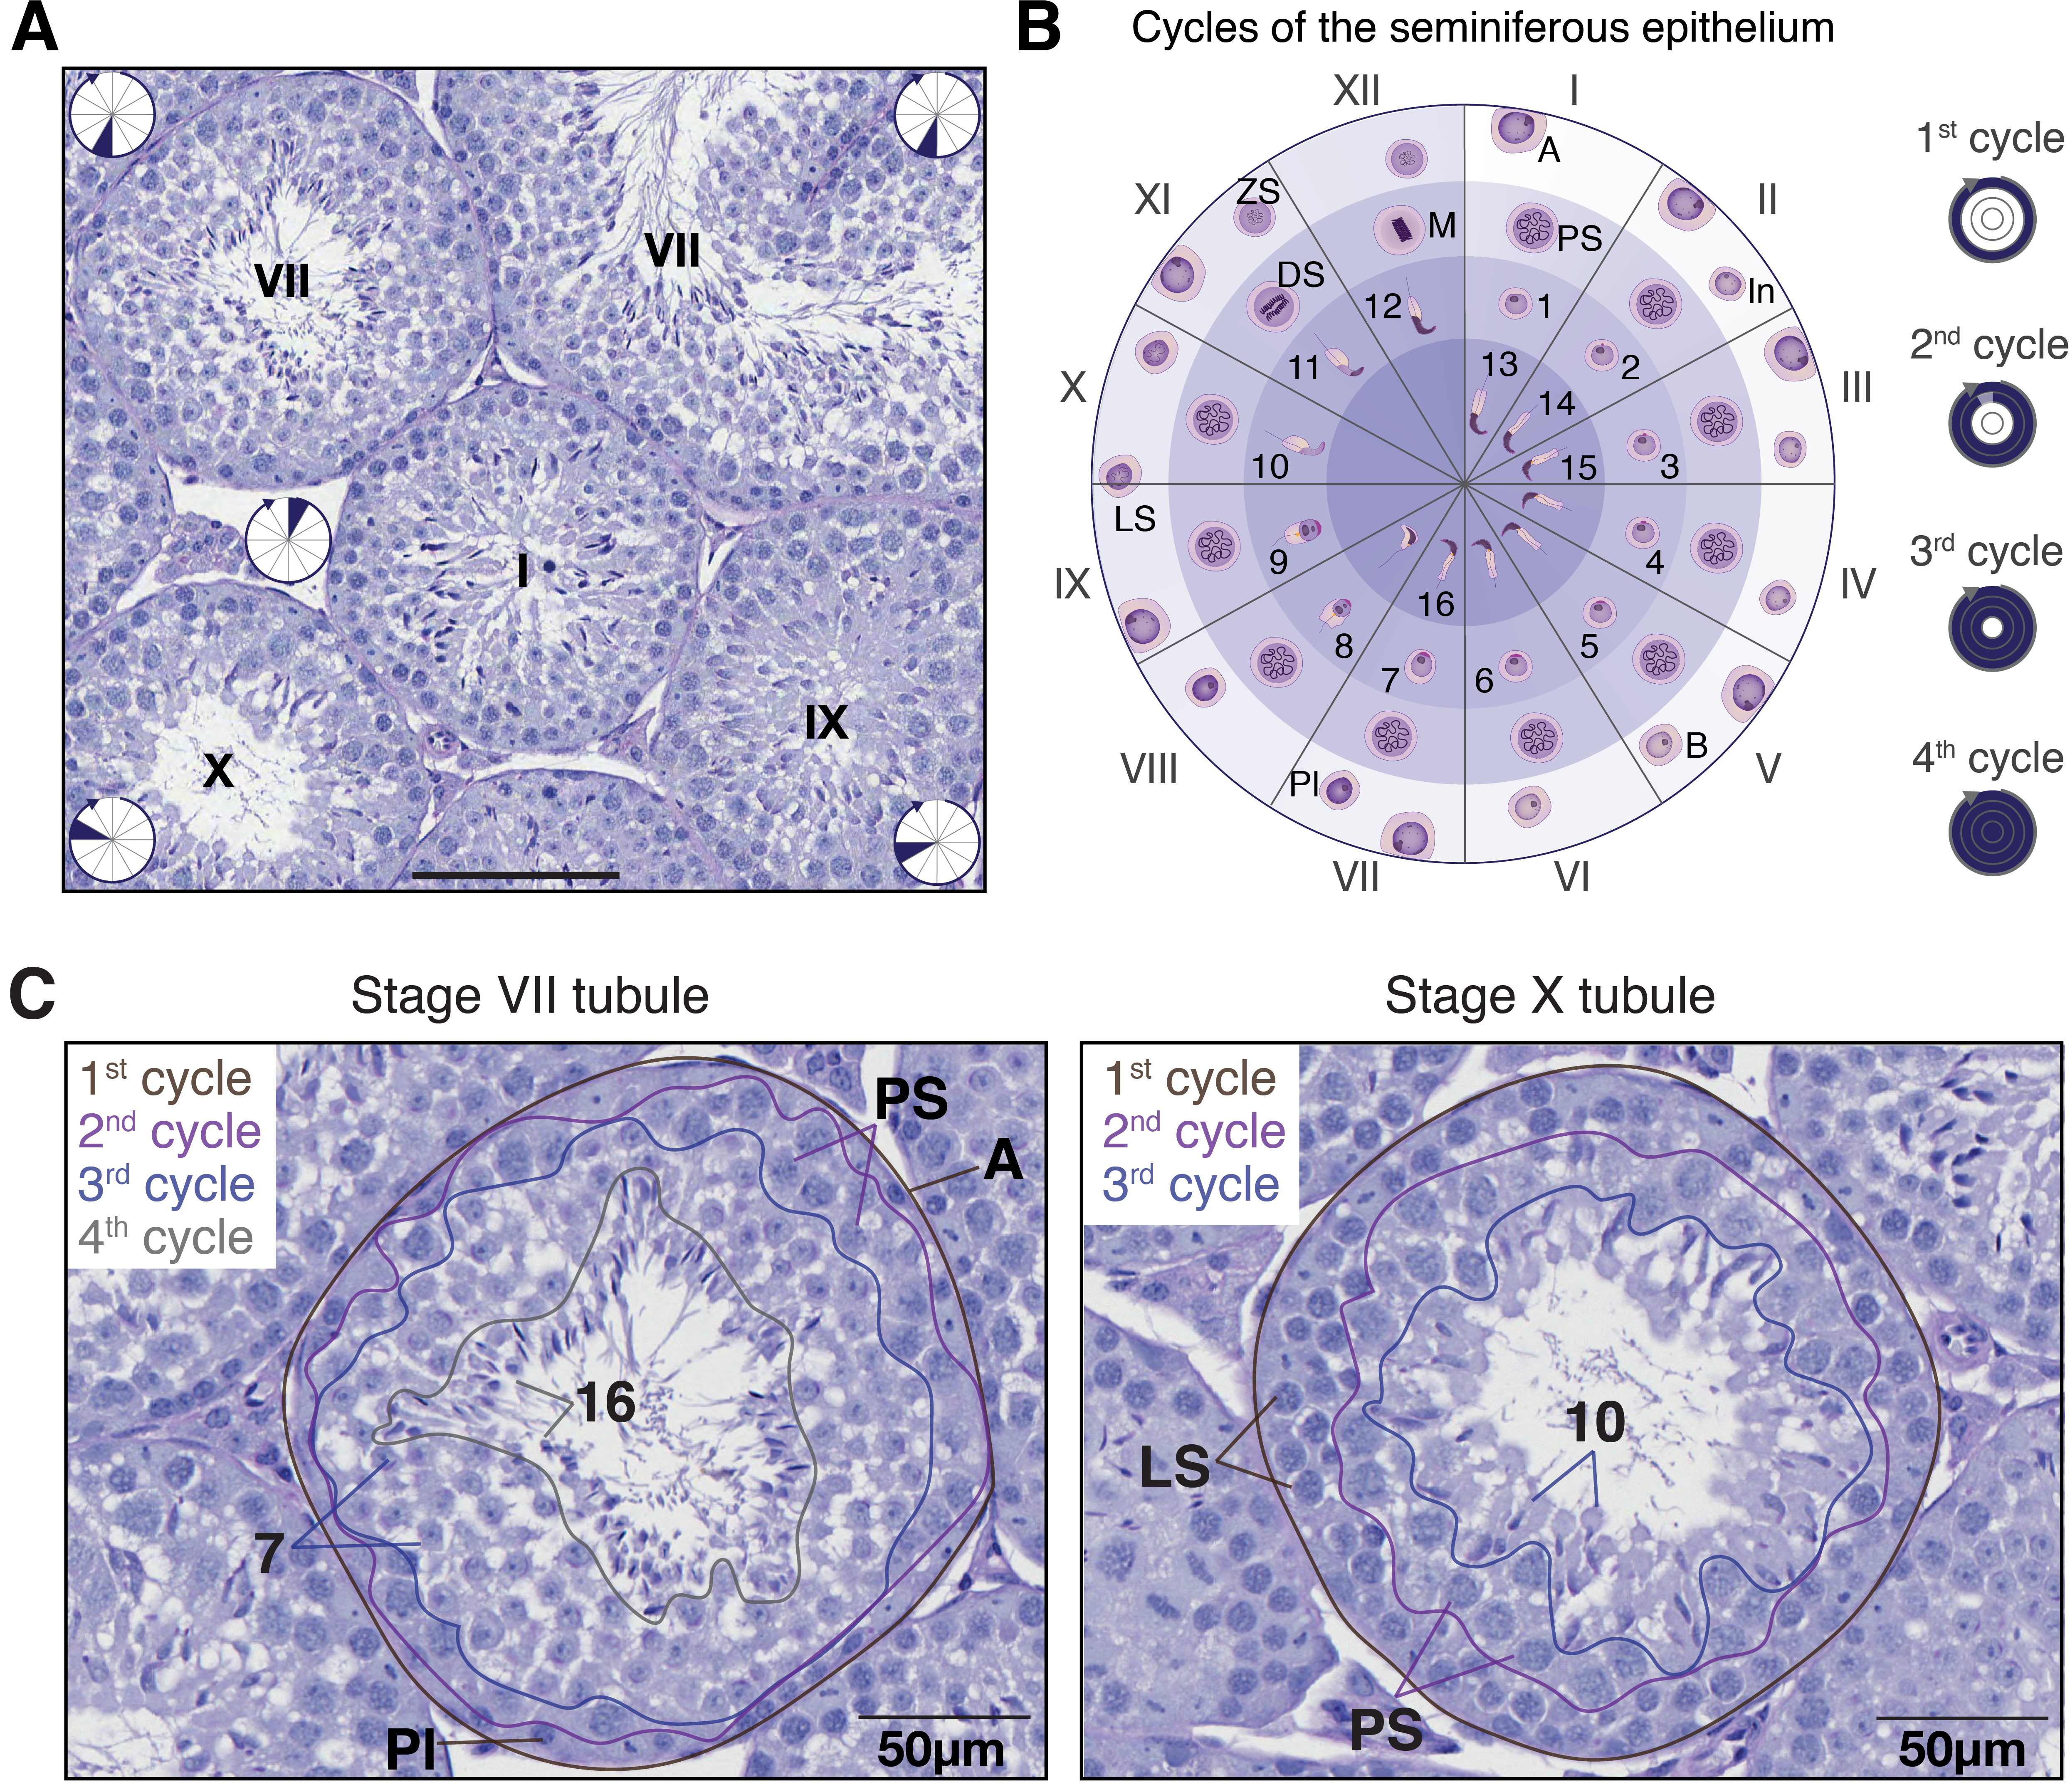
\includegraphics[width=\textwidth]{Fig_1.png}
\caption[Bet-hedging strategy of the $\lambda$-phage]{\textbf{Bet-hedging strategy of the $\lambda$-phage.}\\
The linear genome of the $\lambda$-phage enters the \Gls{Ecoli} host cell and circularises. 
A stochastic decision is made to enter the (i) lytic or (ii) lysogenic cycle where (i) the $\lambda$-phage genome replicates, the $\lambda$-phage particles assemble in the host cell and the cell is destroyed releasing the virions or (ii) the $\lambda$-phage is integrated into the host genome (prophage) and transferred to daughter cells during cell divisions. 
Under stress conditions, the $\lambda$-phage genome is excised from the host genome and enters the lytic cycle.}
\label{fig0:bedhedging}
\end{figure}

In unicellular organisms, \cor{biological noise has been linked to ‘bet-hedging’ strategies, where a sub-optimal fitness landscape is tolerated across a population of cells in order to facilitate an effective response to environmental changes.}. Here, phenotypic heterogeneity facilitates the commitment to alternative cell states in cases of stress (e.g.~nutrient deprivation, temperature fluctuations). 
For example, \Gls{Bsubtilis} either commits to sporulation or competence upon starvation or DNA damage. 
Sporulation describes an irreversible process during which vegetative growth ends and the cell forms endospores that survive the altered environment. 
Competent bacteria on the other hand take up DNA from endospores to repair DNA damage \citep{Schultz2009}. 
The probabilistic and transient activation of competence in a sub-population of \Gls{Bsubtilis} cells is modulated by fluctuations in the competence regulators ComK and ComS. 
An excitable system of negative and positive feedback loops controls the number of cells that reversibly commit to competence while other cells irreversibly execute sporulation \citep{Suel2006}. 
\cor{Variations} in the process of transferring phoshporyl groups across a cascade of regulators maintains a constant probability for cells committing to sporulation under nutrient deprived conditions \citep{Russell2017}. 
A similar phenomenon is observed in \Gls{Ecoli} populations exposed to antibiotics where pre-existing phenotypic heterogeneity allows some cells to resist antibiotic treatment. 
Once regrown, these cells remain sensitive to the antibiotic \citep{Balaban2004}. \\

Similar to phenotypic heterogeneity in unicellular prokaryotes, transcriptional noise facilitates the switching between mating phenotypes in yeast upon exposure to pheromones \citep{Paliwal2007}. 
Comparably, commitment to utilising galactose as a nutrient source is a cell fate transition, which is facilitated by stochastic gene expression \cite{Acar2008}. \\

\cor{In these systems, biological noise introduces variation in mRNA and proteins that increase plasticity for cells to adapt to changeing environments.
However, to control and balance the number of cells that commit to a specific fate, noise needs to be buffered as observed in the regulatory network of feedback loops controlling sporulation and competence.}

\subsection{Development and differentiation}

Similar to bet-hedging strategies in unicellular organisms, noise can facilitate the switch between cell states and the probabilistic induction of differentiation processes \citep{Eldar2010, Chang2008}.
\cor{However, as mentioned above, measuring biological noise in differentiating multi-cellular organisms is challenging and the observed molecular phenotypic variability is a combination of stochastic and deterministic components.} 
It has been shown that transcriptional \cor{variability} increases throughout differentiation \citep{Stumpf2017} and development \citep{Antolovic2017}. 
Dissecting differentiation processes of haematopoietic progenitor cells revealed an increase in transcriptional \cor{variability} directly before cell fate decisions are made \citep{Mojtahedi2016, Richard2016}. 
Once committed, differentiating cell populations collapse in variability and move towards a new attractor state. 
\cor{These studies highlight a possible contribution of molecular variability to cell fate decision event.
However, the observed change in variability within differentiating cell populations is purely correlative and it is not possible, with these experiments, to differentiate between variability causing differentiation or differentiation causing variability.}\\

Studies of recent years proposed that stochasticity in expression \cor{contributes to} early (pre-implantation) embryonic development, and to gastrulation \citep{Dietrich2007}. 
As early as the 4-cell stage embryo, targets of master pluripotency factors Oct4 and Sox2 are heterogeneously expressed \textbf{(Fig.~\ref{fig0:noise_development}, left panel)}. 
This is caused by heterogeneous methylation patterns of \gls{H3R26} induced by \gls{Carm1}, which in turn facilitates the binding of Oct4 and Sox2 to induce pluripotency. 
Cells with unmethylated H3R26 differentiate towards the extra-embryonic trophoectoderm while pluripotent cells form the inner cell mass \citep{Goolam2016}. 
Once the cells compact at \gls{E} 3.5, cells of the \gls{ICM} stochastically express genes to initiate heterogeneity within the cell population \textbf{(Fig.~\ref{fig0:noise_development}, 2\textsuperscript{nd} panel)}. 
Fgf4 driven signal reinforcement controls this heterogeneity to form a salt-and-pepper like cell state pattern at E3.5. 
Positional information and the establishment of gene regulatory networks facilitate the segregation of the epiblast and primitive endoderm lineage at E4.5 \textbf{(Fig.~\ref{fig0:noise_development}, 3\textsuperscript{rd} panel)} \citep{Ohnishi2014}. 
In line with this, scRNA-Seq revealed high levels of \cor{transcriptional variability} in the uncommitted inner cell mass at E3.5 (64-cell stage) in comparison to the E4.5 committed epiblast. 
\cor{Transcriptional variability} increases again upon exit from pluripotency in the E6.5 epiblast while cells of the primitive streak at E6.5 synchronise their expression patterns and \cor{variability} is reduced \textbf{(Fig.~\ref{fig0:noise_development}, right panel)} \citep{Mohammed2017}. \\

\cor{Besides the hypothesis of transcriptional variation contributing to embryonic development, a number of alternative drivers for cell fate decisions the mouse embryo exist\citep{Zhang2018a}. 
For example, in the 8-cell to 16-cell stage embryo, symmetry breaking could be achieved by an interaction between the cell’s position and polarity, its cortical tension, and the orientation of cell division97. 
Maître \emph{et al.} proposed a system where robust self-organization of 8- to 16-cell stage embryos is achieved by differences in contractility between polar and apolar cells, which leads to the internalization of the more contractile apolar cells\citep{Maitre2016}. 
Taken together, it is unclear to which fraction transcriptional variability plays a role in cell fate decision-making and if purely the occurrence of differentiating cells induces transcriptional variation. }

\begin{figure}[!h]
\centering
\includegraphics[width=\textwidth]{Fig_2.png}
\caption[Progression of transcriptional heterogeneity during embryonic development]{\textbf{Progression of transcriptional noise during embryonic development}.\\
From left to right: schematic of mouse embryonic development from the 4-cell stage to early gastrulation at E6.5. 
Cell colours indicate gene expression strength. Variable expression at the 4-cell stage induce commitment to form extra-embryonic lineages or pluripotent cells. 
These pluripotent cells at E3.5 show high expression variability forming the inner cell mass (ICM). 
Cells rearrange to form the epiblast and primitive endoderm at E4.5 while noise levels increase in the epiblast at E6.5 compared to the primitive streak.}
\label{fig0:noise_development}
\end{figure}

While pluripotent stem cells in the mouse embryo commit irreversibly to cell lineages during development, \emph{in vitro} cultured \glspl{mESC} reside in a self-renewing, metastable state \citep{Hayashi2008} and heterogenity within the cell population depends on the growth condition. 
Transcription factor heterogeneity, especially of the pluripotency regulator Nanog, is highest in \gls{LIF}/serum grown cells and allows the Nanog-negative cells to commit to differentiation \citep{Chickarmane2012, Torres-Padilla2014}. 
Heterogeneously expressed genes that show a bimodal distribution in expression counts correlate with each other indicative of the presence of distinct states in mESCs. 
These distinct states show differences in promoter methylation patterns, introducing the role of epigenetic modifications to maintain heterogeneity in mESCs \citep{Singer2014}. 
In-depth analysis of mESCs grown in different media (serum, \gls{2i} and \gls{a2i}) shows the presence of three distinct cell states in the serum grown cells. 
mESCs grown in 2i media show less variability in pluripotency markers but higher heterogeneity in cell cycle related genes \citep{Kolodziejczyk2015cell}. 
From the pluripotent ground state, mESCs can differentiate along somatic lineages via specific differentiation events or noise-induced transitions between attractor states. 
Mathematical modelling has shown that mESCs differentiate stochastically through distinct hidden cell (micro-)states within a defined (macro-)state coupled to an increase in variability \cite{Stumpf2017}.
In contrast to the beneficial features of noise in stem cell differentiation, stochastic events during \gls{iPSC} reprogramming limit the formation of single iPSCs \citep{Hanna2009, Yamanaka2009}. 
It has been shown that probabilistic events dominate in an early phase of reprogramming while the transcription of \textit{Sox2} induces a later, more deterministic, phase \cite{Buganim2012}.\\

\cor{These findings indicate an intrinsic heterogeneity of pluripotent cell populations. 
Extrinsic cues, such as growth medium or signalling networks in the embryo, are needed to control this heterogeneity.
However, it is not clear if this seemingly random expression of pluripotent marker genes is truely stochastic or driven by unobserved regulatory mechanisms.
Hoppe \emph{et al.} challenged the idea of lineage choice by stochastic fluctuations of lineage-specific transcription factors and highlighted, using time-resolved measurements, that these transcription factors are solely reinforcing lineage choice \cite{Hoppe2016}.
Therefore, lineage choice can be initiated by unobserved cues that induce variation in genes expression.} 

\subsection{Stochasticity in immune responses}

Fast and flexible immune responses are only possible within cell populations that show high plasticity and react to a broad spectrum of stimuli. 
Stochasticity in cytokine expression \cor{can} lead to phenotypic variability in the \Gls{Th} cell repertoire and increases the effectiveness to respond upon immune stimuli \citep{Schrom2017}. 
For example, fluctuating expression of the lineage defining cytokines \gls{Ifn}\textgamma{} for Th1 and \gls{Il} 4 for Th2 in small populations of cells drive the cell population towards a Th1 or Th2 cell fate while most cells co-express the lineage defining transcription factors \Gls{Gata} 3 and \Gls{Tbx21} \citep{Fang2013a, Antebi2013}.\\

Furthermore, Shalek \textit{et al.}, 2014 have shown that upon \gls{LPS} stimulation a small subset of dendritic cells become activated much earlier than the rest of the cell population while expressing \gls{Ifn}\textbeta. 
These early responders support the activation of late responding cells via cell-to-cell communication (paracrine signalling) and self-stimulation via autocrine signalling \textbf{(Fig.~\ref{fig0:noise_immune})} \citep{Shalek2014}. 
Likewise, a bimodal (digital) expression of Il2 is detected in \gls{Th} cells after immunisation where the number of Il2 expressing cells scales with antigen level. 
Il2 expressing cells support the activation of surrounding cells via paracrine signalling \citep{Fuhrmann2016}. 
Similarly, digital activation processes can be observed in the \gls{NFkB} signalling pathway. 
The fraction of cells that activate this signalling pathway increase with LPS concentration to avoid strong immune activation at low concentrations of a stimulus \citep{Kellogg2015b}. \\

\cor{While the plasticity and reactivity of immune cell populations is finely tuned by introducing phenotypic heterogeneity, it is not understood how individual cells commit to each phenotype. 
In part, stochastic expression introduces molecular phenotypic variability that in turn is tightly controlled by external and internal signalling networks. 
It will therefore be crucial to study the behaviour of immune cells while incorporating their spatial location which might allow the prediction of each cell's phenotype\cite{Battich2015}.}

\begin{figure}[!h]
\centering
\includegraphics[width=\textwidth]{Fig_3.png}
\caption[Early responders are important for homogeneous immune activation]{\textbf{Early responders are important for homogeneous immune activation.}\\
Within a population of immune cells (e.g.~\gls{DC}, \gls{Th} cells), a sub-population either show higher response strength or induce the production of cytokines such as \gls{Il}2 or \gls{Ifn}\textbeta. 
These early responders induce activation of surrounding cells via paracrine signalling and self-stimulation via autocrine signalling.}
\label{fig0:noise_immune}
\end{figure}

\vspace{-5mm}

\subsection{Tissue development and homeostasis}

Coping with the influence of biological noise is important for regulated tissue development and homeostasis. 
An early study showed that in order to minimise the effect of stochasticity in development, plants express heat-shock protein 90 to stabilise regulators of growth and development \citep{Queitsch2002}. 
Furthermore, redundancy in the \Gls{Celegans} intestinal gene regulatory network buffers variability in the down-stream master regulator \textit{elt-2}. 
Once highly connected regulators of this network are removed, phenotypic variation arises from bimodal expression of \textit{elt-2} \citep{Raj2010}. 
The cooperation of positive and negative feedback loops in these highly connected regulatory networks ensure robust expression of key developmental genes \citep{Ji2013}. 
Other models have been proposed in which noise helps to form sharp boundaries between neighbouring domains \citep{Zhang2012}. 
Contact based adhesion and repulsion between cells sharpens narrow transition regions by sorting cells within a tissue across small scales. 
Noise-driven cell state plasticity on the other hand allows cells to switch states and therefore helps narrow a wider transition region \citep{Wang2017}. 
The plasticity to migrate within a population of cells also allow the correction of sensing errors. 
These errors are induced by either too strong or too weak responses of individual cells to a signalling gradient \citep{Camley2017}.\\

While the cell division rate within tissues is higher during development, tissue homeostasis is maintained by stochastic events that balance cell division and apoptosis \citep{Ranft2010}. 
The effect of noise on maintaining tissue homeostasis has been studied in a diverse set of organs. 
In fat tissue, a complex system of signalling feedback loops controls protein abundance noise to induce differentiation at a low rate but prevents stochastic de-differentiation \citep{Ahrends2014}. 
To maintain coordination in liver function, longer mRNA lifetimes of bursty genes and polyploidy reduce noise in gene expression \citep{BaharHalpern2015}. 
Another mechanism to achieve tissue-wide expression responses involves spatial coordination of stochastically expressing cells in the pituitary gland \citep{Featherstone2016}. 
Spatially constrained signalling events have also been demonstrated to play a role in maintaining colonic crypt cell type diversity. 
Per crypt, eight stem cells differentiate into a defined ratio of cell types. To reduce noise in this process, lateral inhibition within a commitment zone reduces the number of differentiated goblet cells and following slower dispersive migration as well as decreased division rates of goblet cells ensures a distinct 1:3 ratio to enterocytes across all crypts \textbf{(Fig.~\ref{fig0:noise_tissue})} \citep{Toth2017}.

\cor{In sum, phenotypic heterogeneity in tissues can arise from stochastic expression driven by noise.
To control for correct tissue responses, signalling networks are in place to modulate this variation. 
In most studies, individual signalling networks and few molecular read-outs were chosen to understand the variation observed within tissues.
However, a combination of multiple regulatory signalling events control cell fate within tissues and disentangling the individual components has not been feasible.}

\begin{figure}[!h]
\centering
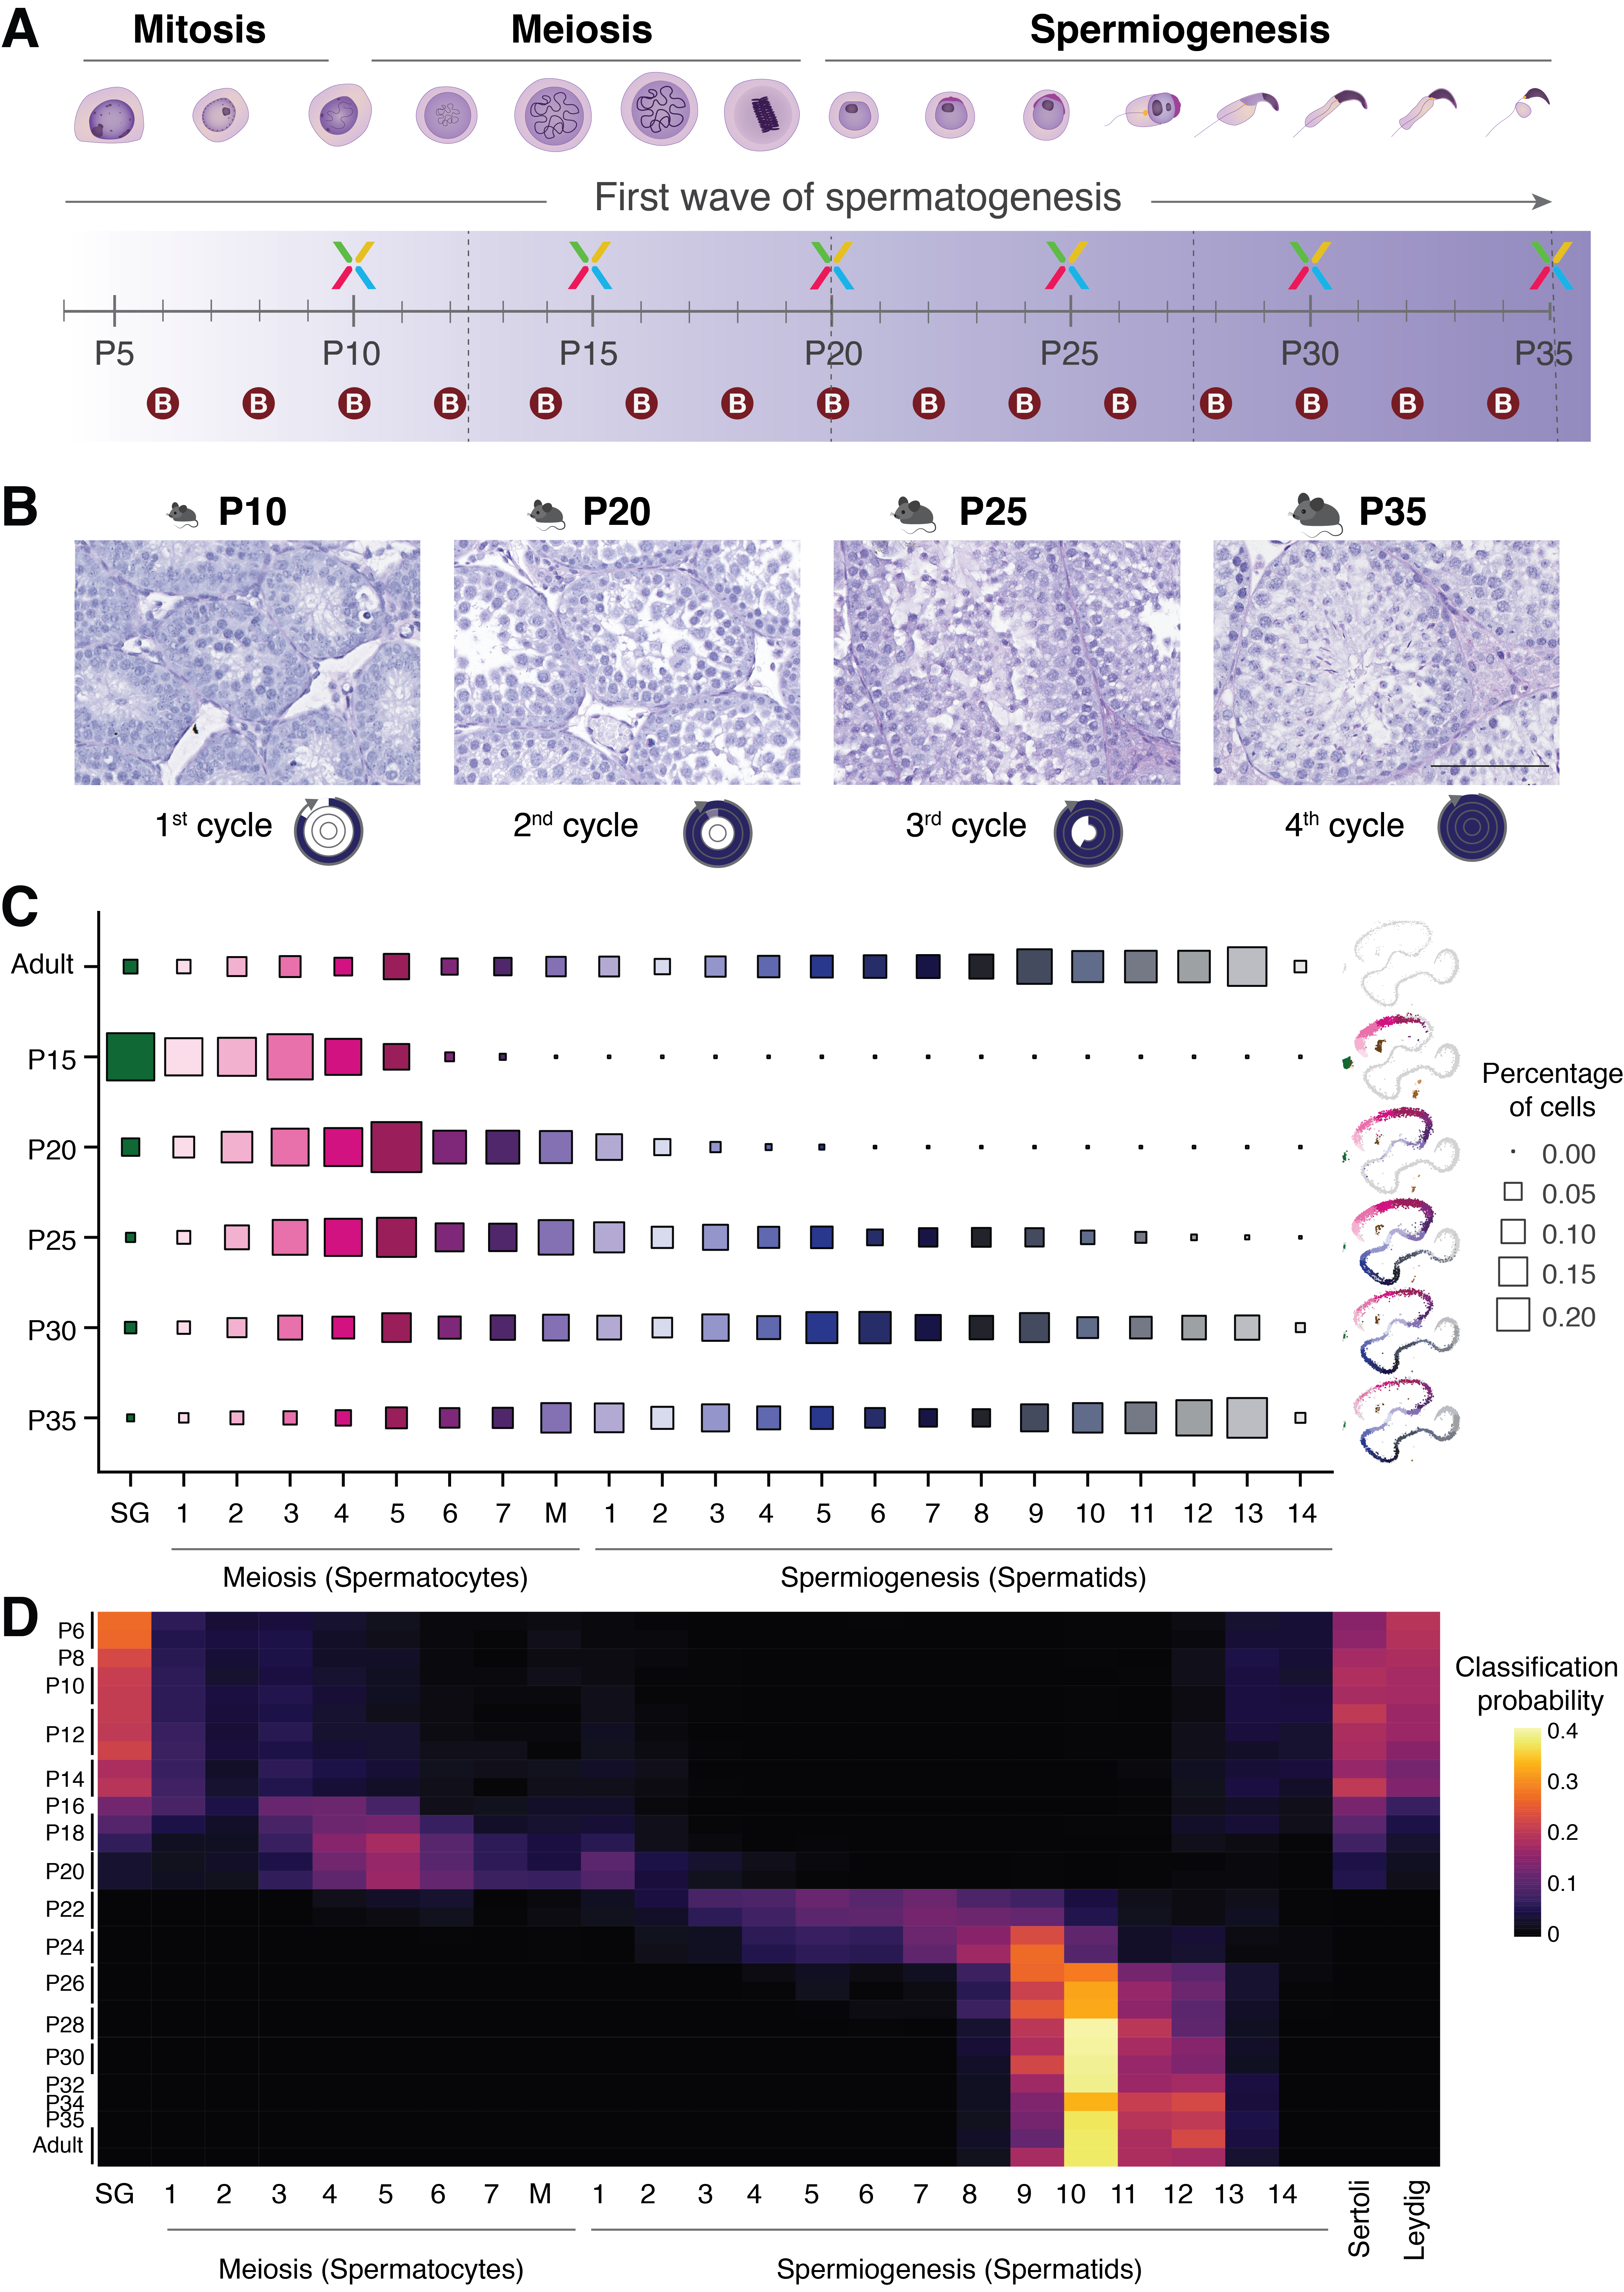
\includegraphics[width=\textwidth]{Fig_4.png}
\caption[Buffering of noise in the colonic crypt]{\textbf{Buffering of noise in the colonic crypt.}\\
Each colonic crypt harbours 6-8 stem cells that divide to form stem cells and progenitors cells. 
Early commitment of progenitor cells to cell fates (e.g.~goblet cells or enterocytes) leads to crypt-to-crypt heterogeneity due to commitment noise (left panel). 
Lateral inhibition within a restricted zone (commitment zone) allows cell fate switching and therefore buffers the crypt-to-crypt heterogeneity (middle panel). 
Migration of goblet cells after the commitment zone buffers the stochastic occurrence of goblet cell or enteroctye patches within the crypt and allows a constant ratio of 1:3 goblet cells to enterocytes in each crypt (right panel). 
Adapted from \citep{Toth2017}.}
\label{fig0:noise_tissue}
\end{figure}

\subsection{Evolution}

As discussed above, biological noise \cor{can be} beneficial for cell fate commitment \cor{but} needs to be \cor{controlled} to allow coordinated expression in cell populations. 
During evolution, a trade-off between cellular plasticity, the expression responsiveness during environmental changes, and robust expression formed. 
Natural selection acts on genetically controlled expansions of quantitative phenotypes, which\cor{, in part, are} derived from biological noise \citep{Eldar2010}. 
For example, \cor{variable} expression of stress response genes allows a cell population to adapt to changing environments \citep{Lopez-Maury2009}. 
Specifically, the expression of genes controlled by TATA-box containing promoters shows strong divergence between species \citep{Tirosh2006}. 
To control for robust expression levels once selection becomes stabilising, noise levels are reduced \citep{Lopez-Maury2009, Eldar2010, Pires2016}. \\

Lehner, 2008 discussed specifically evolutionary selection to minimise noise in genes that show harmful phenotypic effects upon alteration ("dosage-sensitive genes"). 
These genes show low expression \cor{variability} to reduce the probability of altered expression and also lower expression divergence between species \citep{Lehner2008}. 
Furthermore, essential genes tend to cluster in the genome in regions with persistent open chromatin to reduce \cor{the effect of} noise \citep{Batada2007}. 
In line with this, the promoters of core cellular components show a decoupling between expression plasticity and expression \cor{variability}, which indicates that responsiveness in expression is not a general attribute of high expression \cor{variability} \citep{Lehner2010a}. \\

In unicellular populations, \cor{it has been proposed that the contribution of noise on molecular phenotypic variability} evolutionarily increased as a form of rudimentary regulation \citep{Wolf2015}. 
As a consequence, phenotypic heterogeneity increases the adaption rate of cell populations to extreme environments \cite{Bodi2017}. 
Conversely, in multicellular organisms, collections of cells need to respond in a coordinated manner. 
It has therefore been proposed that nuclear compartmentalisation in higher organisms reduces noise by mRNA retention at the nuclear membrane \citep{Battich2013, Stoeger2016}.

\cor{In most cases, cells in an unperturbed state have been profiled to decipher evolutionary selection acting on variability in gene expression.
However, in fluctuating environments where the averaged protein abundance across a cell population is far from the optimum, variability in expression leads to some cells expressing protein levels closer to the optimum. 
By contrast, in stable environments, noise in gene expression can be deleterious by leading to suboptimal growth conditions for many cells\cite{Schmiedel2018,Duveau2018}.
It is therefore crucial to discuss the fitness effect of changes in molecular variability in the context of fluctuating as well as stable environments.}

\subsection{Cancer}

While biological noise \cor{can contributeto } the adjustment of cells to new microenvironments, errors in the form of gene mutations induce transitions from healthy cells towards a cancer attractor state \textbf{(Fig.~\ref{fig0:cancer})} \citep{Marusyk2012}. 
Non-genetic heterogeneity supports the phenotypic adaptation to the new attractor state \citep{Jia2017}. 
The emergence of non-genetic heterogeneity in tumours is coupled to epigenetic dysregulation that allows the survival of cancer cells \citep{Timp2013}. 
Furthermore, it has been proposed that genome wide intra-sample methylation heterogeneity is increased in chronic lymphoitic leukemia increasing cancer cell plasticity in the search for new attractor states \citep{Landau2014}. 
Increased variability in expression can also be observed for more aggressive cancer sub-types across multiple patients \citep{Ecker2015}. \\

An important consequence of \cor{increased} phenotypic heterogeneity in cancer cells is the fractional killing of cell populations upon drug treatment \textbf{(Fig.~\ref{fig0:cancer})} \citep{Flusberg2015}. 
\cor{Variability} in proteins mediating \Gls{TRAIL} induced apoptosis leads to the survival of small fractions of cells \citep{Spencer2009}, which could consequently repopulate the tumour environment. 
Similarly, the stochastic acquisition of DNA damage upon cisplatin exposure introduces heterogeneity in the up-regulation of p53. 
Slow up-regulation leads to cell cycle arrest and inhibits apoptosis while only fast up-regulation leads to cell death \citep{Paek2016}. 
In patient derived melanoma cells, sporadic expression of resistance markers forms a rare cell population that grows into resistant colonies after treatment. 
While pre-resistant cells do not display epigenetic marks and are therefore close to the non-resistant ground state, treatment induces large epigenetic reprogramming, forming stable resistant cancer colonies \citep{Shaffer2017}. 
To tackle this problem, combinatorial therapies have been proposed to reduce variability and fractional killing in cancer cell populations \cite{Paek2016, Roux2015}.\\

\cor{These studies propose a contribution of non-genetic heterogeneity, potentially induced by the loss of noise control, to cancer onset and inefficient treatment response.
However, cancer is a heterogeneous disease that develops in a multi-step process involving disregulation in various cellular systems. 
Therefore, and similar to molecular phenotypic variability in embryonic development, the observed non-genetic heterogeneity can be a phenotypic consequence rather than a driver for cancer onset. }

\begin{figure}[!h]
\centering
\includegraphics[width=\textwidth]{Fig_5.png}
\caption[Heterogeneous cell states and cell responses in cancer development]{\textbf{Heterogeneous cell states and cell responses in cancer development.}\\
Stochasticity in expression introduces non-genetic heterogeneity that supports the adaptation of cancerous cells. 
Cancer progresses to form a collection of cells with divergent expression patterns. 
This phenotypic heterogeneity leads to fractional killing during treatment and cancer recurrence.}
\label{fig0:cancer}
\end{figure}

\newpage

\subsection{Ageing}

Similarly to the onset of cancer, destructive roles of biological noise have been reported during organismal ageing. 
Previously, it has been debated whether expression noise changes during the lifespan of animals \cite{Bahar2006, Warren2007}. 
While these initial studies only used small panels of genes, transcriptional profiling of single cells led to the discovery of a destabilised immune activation programme in CD4\plus{} T cells due to increased expression noise \cite{Martinez-jimenez2017}. 
Similarly, transcriptional noise increases with age in human pancreas coupled to an increased stress signature and atypical hormone expression \citep{Enge2017}. 
For further discussion of age-related effects on transcriptional noise, see \textbf{Chapter 2}. \\


\begin{table}[hb	]
\centering
\caption{Positive and negative effects of biological noise on cellular systems.}
\label{table:effects_noise}
\begin{tabular}{l l l}
\toprule
\toprule
\textbf{System} & \textbf{Friend} & \textbf{Foe} \\ 
\midrule
\midrule
Unicellular organism & Bet-hedging & \\
\midrule
Development and & Probabilistic induction  & \\
differentiation & of cell differentiation & \\
\midrule
Immune response & Plasticity in immune response & \\
 & Control of response strength &   \\
\midrule
Tissue development  & Low cell differentiation rate & Non-uniform development \\ 
and homeostasis &  & Uncontrolled tissue response \\
\midrule
Evolution & Adjustment to  & Non-uniform, stabilising expression \\ 
& fluctuating environment & Uncontrolled tissue responses \\
\midrule
Cancer &  & Phenotypic adaption to cancer state \\
& & Fractional killing of cancer cells \\
\midrule
Ageing &  & Unsynchronised immune response \\
& & Increased stress signatures \\ 
\bottomrule
\bottomrule
\end{tabular}
\end{table}

\newpage
%!TEX root = ../intro.tex
%******************************
%	 Sources of expression noise
%*****************************

\section{Sources of expression noise} 

\cor{Molecular phenotypic variability} across homogeneous populations of cells \cor{can arise} from intrinsic and extrinsic noise, \cor{and deterministic components} (see \textbf{Box 1} on page \pageref{box1}). 
While intrinsic noise is promoter-specific and therefore induces uncoordinated variation in RNA or protein expression between individual genes, extrinsic noise globally influences gene expression across multiple cells and therefore leads to co-variation across larger sets of genes. 
Here, I give an overview on the different sources of intrinsic and extrinsic noise in a variety of biological systems.

\subsection{Intrinsic noise}

Intrinsic noise in cell populations arises from stochasticity in biochemical reactions that lead to the synthesis of mRNAs (transcription) and proteins (translation) within individual cells. 
Regulatory features on the genomic, epigenetic, transcriptional and translational level influence \cor{and control} the strength of intrinsic noise (for an overview see \textbf{Fig.~\ref{fig0:overview_intrinsic}}).

\begin{figure}[!h]
\centering
\includegraphics[width=0.9\textwidth]{Fig_6.png}
\caption[Regulatory features that modulate expression noise]{\textbf{Regulatory features that modulate expression noise.}\\
Promoter sequence, number of transcription factor (TF) binding sites (TFBS), number of transcriptional start sites (TSS), enhancer elements, RNA polymerase II (RNAPII) loading, DNA methylation, nucleosome positioning, histone modifications, polycomb repressive complex binding, \glspl{miRNA}, nuclear export of mRNA, ribosome binding and blockage via stem loop formation are features that induce gene-specific intrinsic noise.}
\label{fig0:overview_intrinsic}
\end{figure}

\subsubsection{DNA features}

One of the key regulatory steps prior to RNA synthesis is the binding of \glspl{TF} to specific DNA sequences within the regulatory region (promoter) of a gene which then triggers the controlled production of primary RNA transcripts from the DNA of this gene \citep{Latchman1997}. 
Mutations in the DNA sequence such as \glspl{SNV} can alter the binding affinity of TFs and therefore the rate at which a gene is expressed \textbf{(Fig.~\ref{fig0:DNA_features})}. 
A systematic study of the \gls{TDH3} gene expression in yeast found that mutations in known \glspl{TFBS} decrease mean expression and increase expression noise. 
Moreover, Metzger \textit{et al.}, 2015 \cor{proposed} that evolutionary selection removes mutations that increase expression noise and that SNVs with large effects on expression noise show the lowest frequency within sampled yeast strains \citep{Metzger2015}. 
\cor{However, the authors examined one promoter in stable environmental conditions. 
How selection on mutations that induce variability in expression works in more complex systems and across multiple promoters is still unexplored.}\\

One of the most widely studied DNA motifs in relation to transcriptional noise is the TATA-box motif in promoters. 
Generally, TATA-box containing promoters show high levels of transcriptional noise \textbf{(Fig.~\ref{fig0:DNA_features})} \citep{Faure2017}, possibly due to a simple activation cycle containing one or few inactive states \citep{Zoller2015}. 
Moreover, TATA-box containing genes show an increased interspecies variability \citep{Tirosh2006} and higher spontaneous mutational variation \citep{Landry2007}, indicating an increased evolvability of these particular genes. 
In an early study, Raser \textit{et al.}, 2004 studied the noisy expression controlled by the budding yeast \gls{PHO5} promoter. 
This promoter contains the TATA-box motif and it has been shown that transcriptional noise is reduced when a mutational modification decreases the TATA-box strength \citep{Raser2004}. 
A more recent study confirmed this result and found mutations in yeast promoters that eliminate the TATA-box motif which lead to reduced noise levels for these genes \citep{Hornung2012}. 
\cor{The TATA-box is therefore one genomic feature that can differentiate between genes with variable and stable expression and are enriched amongst stress response genes, which support their role in early adjustment to changing environmental conditions \citep{Lopez-Maury2009}.}\\

\cor{However, a} possible confounding factor for the increased noise of TATA-box containing promoters is the number of TFBSs. 
Tirosh \textit{et al.}, 2006 detected a two-fold enrichment of TFBSs in TATA-box containing promoters \citep{Tirosh2006}. 
A later study showed that transcriptional noise scales with increased numbers of TFBSs \textbf{(Fig.~\ref{fig0:DNA_features})} \citep{Sharon2014}. 
Furthermore, TATA-box containing genes lack enhancing histone marks and their increased variability in expression can therefore be explained by repressed chromatin \citep{Choi2008} (see \textbf{Section \ref{sec0:epigenetic}}).  

\begin{figure}[!h]
\centering
\includegraphics[width=0.9\textwidth]{Fig_7.png}
\caption[Features of the DNA sequence induce expression noise]{\textbf{Features of the DNA sequence induce expression noise.}\\
Mutations of the transcription factor (TF) binding site (TFBS), the presence of a TATA box, increase number of TFBSs, reduced number of transcriptional start sites (TSSs) and reduced copy number of genes can induce transcriptional noise.}
\label{fig0:DNA_features}
\end{figure}

Promoters can be classified based on their shape as narrow, with few \glspl{TSS} that predominantly control tissue-specific gene expression, and broad promoters with larger numbers of TSSs that control the expression of house keeping genes. 
Mutations that alter the shape of promoters increase transcriptional \cor{variability} \citep{Schor2017a}. 
Furthermore, promoters with one or few TSS show higher levels of expression variability \textbf{(Fig.~\ref{fig0:DNA_features})} \citep{Faure2017}.

\newpage

In addition to \glspl{SNV}, \glspl{CNV} (usually defined as copy number variability of regions $\geq$ 1kb in comparison to a reference genome) in parts of the genome influence gene expression and contribute to, for example, schizophrenia and autism \citep{Gamazon2015}. 
Combined analysis of DNA and RNA has shown that genes with low copy number tend to be more noisily expressed compared to genes encoded by multiple copies \textbf{(Fig.~\ref{fig0:DNA_features})} \citep{Dey2015}. 
In the context of monoallelic expression, genes located on the X chromosome show increased mRNA half-life which in turn increases transcript stability and reduces noise to levels of autosomal genes \citep{Faure2017}.\\

\cor{In sum, these findings highlight that multiple correlated genomic features are associated with modulating noise. 
It is therefore challenging to disentangle the individual underlying sources of transcriptional variability. }

\subsubsection{Epigenetic factors}
\label{sec0:epigenetic}

Epigenetic research is defined as "the study of changes in gene function that are mitotically and/or meiotically heritable and that do not entail a change in DNA sequence" \citep{Wu2001}. 
Epigenetic factors are generally described as DNA methylation at \gls{CpG} dinucleotides, histone modifications and nucleosome positioning  \citep{Portela2010}. 
\textbf{Table \ref{tab0:epigenetic}} summarises the relationship between epigenetic features and \cor{variable} gene expression. \\

\Gls{CGI} are genomic sites of more than 200 bases with a GC content of more than 50\% and are usually unmethylated. 
Methylation of CGIs in promoters is linked to gene silencing while DNA methylation in gene bodies facilitates transcription \citep{Portela2010}.  
Recently, the presence of CGIs in gene bodies but also at the TSS and in promoter regions was linked to a reduction in transcriptional \cor{variability} \citep{Faure2017}. 
\cor{Morgan and Marioni, 2018 further distinguished between gene promoters associated with short and long CGIs.  
Similar to the presence of TATA-box motifs as described above, the length of CGIs in promoter regions controls how variably a gene is expressed. 
Genes associated with short CGIs tend to be more variably expressed and allow an early response to stimulation, exemplified by observations in mouse bone-marrow derived dendritic cells and human breast cancer cells \citep{Morgan2018}.
However, it is not clear whether the length of CGIs is the sole driver for variable gene expression or how multiple genomic features work together to induce transcriptional variability.} \\

Modifications of histones induce the \cor{opening} or repression of chromatin and  therefore indirectly modulate gene expression \citep{Suganuma2011}. 
In an extensive study to link histone modifications to transcriptional \cor{variability}, Faure \textit{et al.}, 2017 detected several histone modifications in promoter/core promoter motifs, at the TSS and in gene bodies that increase or decrease \cor{variability}. 
The repressive \gls{H3K27me3} mark is linked to higher \cor{variability} when present at the TSS, in promoters and in gene bodies. 
The enhancer related \gls{H3K4me1} mark only increases \cor{variability} when present at the TSS and in the core promoter sequence while the repressive \gls{H3K9me3} mark increases \cor{variability} when present in the promoter motif. 
The activating marks \gls{H3K4me3}, \gls{H3K9ac} and \gls{H3K36me3} are linked to low levels of \cor{variability} when present in gene bodies. 
In addition to these single features, bivalent promoters that carry the repressive \gls{H3K27me3} and enhancing \gls{H3K4me3} marks show high levels of transcriptional \cor{variability} \citep{Faure2017}.
\cor{Here and in Morgan and Marioni, 2018, the authors profiled molecular phenotypic variability in "homogeneous" populations of \glspl{mESC} as proxy for transcriptional noise.
While the effect of fluctuation in cell-cycle stages was regressed out, unobserved variation in, for example, the differentiation potential of mESCs in serum grown medium \cite{Kolodziejczyk2015cell} could still exist.
It is therefore difficult to use scRNA-Seq data to study the true underlying effect of transcriptional noise on the overall observable phenotypic variability.}\\ 

\cor{One suggestion why bivalent promoters show high transcriptional variability was brought forward by Kar \emph{et al.}, 2017.
Here, the authors studied the function of \glspl{PRC} in mESCs.}
PRCs are epigenetic modifiers of histones that repress transcription of developmental genes \citep{Chittock2017} and they can bind together with active \gls{RNAPII} to bivalent promoters. 
Switching between the repressed and active states introduces gene expression variability across a population of cells \cite{Kar2017}.
\cor{However, bulk measures were used to identify the bivalency of promoters.
That leaves the possibility that in a fraction of cells the promoter resides in an open state while in other cells the promoter is repressed. 
This highlights the fact that bulk measures might not be suitable to obtain a correct measure of promoter states in cell populations that could contain unobserved cell state heterogeneity.} \\

Chromatin is the packaged state of DNA within the nucleus and its central elements are nucleosomes. 
Nucleosomes are combinations of eight of the four histones (H3, H4, H2A, H2B) around which 147 bases of DNA twist. 
An array of histone modifying enzymes exist that regulate the opening or closing of the chromatin; termed heterochromatin and euchromatin, respectively \citep{Kouzarides2007}. 
Tirosh \textit{et al.}, 2008 showed that promoters with high nucleosome occupancy close to the TSS tend to display a high range of expression levels across varying conditions (transcriptional plasticity). 
Distant nucleosome-rich regions are on the other hand associated with low transcriptional \cor{variability} \citep{Tirosh2008}. 
Nucleosome covered promoters display shorter transcriptional rates, which in turn explains increased transcriptional \cor{variability} for these promoters \cite{Dey2015}. 
Single-cell measures indicate cell-to-cell variations in nucleosome positioning around the \textit{PHO5} promoter upon stress induction. 
Even in the non-stressed state, a small fraction of cells exhibit nucleosome free regions at the promoter which explains low and possibly noisy expression of \textit{PHO5} \citep{Small2014}.
\cor{This observation again highlights the lack of resolution when using bulk measures to profile the promoter architectures in cell populations.
However, current single-cell technologies to profile epigenetic marks lack throughput and are influenced by high levels of technical noise.
The observed variations in nucleosome occupancy could therefore be driven by technical variation.} \\

Boundaries between heterochromatin and euchromatin are controlled by boundary elements, such as the transcription factor \Gls{CTCF}, that recruit chromatin modifying factors \citep{Kouzarides2007}. 
CTCF also regulates transcription by activating or repressing promoters and regulates distant chromatin interactions \citep{Kim2015a}. 
Recent studies suggest that long-range enhancer-promoter interactions modulate transcriptional noise. 
Interference of CTCF-mediated enhancer-promoter contact either by CTCF knock-out or CTCF-binding site deletion leads to increased expression variability in selected genes \citep{Ren2017}. 
\cor{This study however only profiled protein abundance of few genes and did not correct for changes in mean expression that are highly correlated with changes in variance \cite{Brennecke2013}.}
Enhancers are cis-regulatory elements of non-coding DNA containing TFBSs that regulate the expression of neighbouring genes \citep{Blackwood1998}. 
Genes within super-enhancer loci, a region with multiple enhancers, control pluripotency master regulators and show high levels of variability in expression down-stream targets of these master regulators show similar co-variation across mESCs \citep{Faure2017}.

\newpage

\begin{table}[hb	]
\centering
\caption{Epigenetic control of transcriptional noise}
\label{tab0:epigenetic}
\begin{tabular}{l l c c}
\toprule
\toprule
 & Feature & \cor{Variable} & Stable \\ 
\midrule
\midrule
\multirow{3}{*}[-2pt]{DNA methylation} & CGIs &  & \checkmark{} \\
\cmidrule{2-4}
& Short CGIs & \checkmark{} &  \\
\cmidrule{2-4}
& Gene body methylation &  & \checkmark{} \\
\midrule
\multirow{7}{*}[-2pt]{Histone modification} & H3K27me3 (TSS, promoter, gene body) & \checkmark{}  & \\
\cmidrule{2-4}
& H3K4me1 (TSS, promoter) & \checkmark{}  & \\
\cmidrule{2-4}
& H3K9me3 (promoter) & \checkmark{}  & \\
\cmidrule{2-4}
& H3K4me3 (gene bodies) &  & \checkmark{}\\
\cmidrule{2-4}
& H3K9ac (gene bodies) &  & \checkmark{} \\
\cmidrule{2-4}
& H3K36me3 (gene bodies) &  & \checkmark{} \\
\cmidrule{2-4}
& H3K27me3 and H3K4me3 & \checkmark{}  & \\
\midrule
\multirow{3}{*}[-2pt]{Nucleosome position} & Nucleosome rich promoters & \checkmark{} & \\
\cmidrule{2-4}
& Distant nucleosome rich regions &  & \checkmark{} \\
\cmidrule{2-4}
& Deletion of nucleosome remodelling complexes & \checkmark{}  & \\
\midrule
\multirow{7}{*}[-2pt]{Genome architecture} & CTCF knock-out & \checkmark{} & \\
\cmidrule{2-4}
& CTCF binding site depletion & \checkmark{} & \\
\cmidrule{2-4}
& Clustered genes &  & \checkmark{} \\
\cmidrule{2-4}
& Nuclear-lamina associated genes & \checkmark{} & \\
\bottomrule
\bottomrule
\end{tabular}
\end{table} 

Moreover, the positioning of genes on the genome controls expression noise with densely clustered genes being less \cor{variably} expressed in comparison to non-clustered genes \citep{Kustatscher2017}. 
Additionally, genes positioned next to “noisy” genes display higher levels of transcriptional variability compared to genes that are located in proximity to “stable” genes \citep{Kar2017}. 
Expression \cor{variability} is also increased for genes that are located in a repressed neighbourhood, namely active genes in constitutive nuclear lamina-associated domains \citep{Faure2017}.
\cor{This finding again highlights that genes associated with repressed chromatin display higher transcriptional variability compared to genes associated with open chromatin.
Single-cell measures are needed to provide an insight into whether this effect is driven by so called "leaky" expression from closed promoters of if heterogeneous promoter states can be observed.}

\subsubsection{Transcriptional features}

Transcription is initiated by TFs binding to specific regulatory DNA sequences followed by recruitment of RNAPII and RNA synthesis. 
As discussed above, promoter architecture, namely the location and accessibility of TFBS and RNAPII binding sites, dictates mean expression and transcriptional \cor{variability}. \\

In bacteria, the intracellular physical distance between TF source and the promoter sequence influences expression variability. 
TF expression proximal to their target genes results in less \cor{variable} expression compared to TF expression which occurs distant to the promoter sequence \citep{Goni-Moreno2017}. 
Once TFs bind to their target sequence, Carey \emph{et al.}, 2013 showed that the mean expression to \cor{expression variability} ratio is promoter dependent while in the majority of cases, \cor{variability} negatively scales with mean expression \citep{Carey2013}. \\

Similar to TF binding dynamics, the assembly of RNAPII complexes modulates transcriptional noise. 
An early study identified the connection between paused RNAPII and synchronous expression of target genes. 
Genes without pre-loaded RNAPII show more stochastic activation patterns \citep{Boettiger2009}. 
This finding has later been confirmed using scRNA-Seq data where increased variability was detected for genes with actively transcribing RNAPII across the full range of expression levels \textbf{(Fig.~\ref{fig0:RNAPII})} \citep{Day2016}.
\cor{However, genes with pre-loaded RNAPII also have a higher CpG content and are depleted for TATA-box elements \cite{Day2016}. 
Once again, the correlation between genomic factors and their individual associations with variation creates a challenge for disentangling their specific effects on molecular phenotypic variation.
Alternatively, this may also represent multiple regulatory layers that combine to modulate noise. }\\

\begin{figure}[!h]
\centering
\includegraphics[width=0.7\textwidth]{Fig_8.png}
\caption[RNAPII pausing reduces transcriptional noise]{\textbf{RNAPII pausing reduces transcriptional noise.}\\
Left: Pre-loaded RNA polymerase II (RNAPII) allows direct transcription upon transcription factor (TF) binding. 
Right: RNAPII recruitment induces gene expression variability.}
\label{fig0:RNAPII}
\end{figure} 

\newpage

\subsubsection{Post-transcriptional and translational features}

After synthesis, pre-RNAs are polyadenylated and spliced to form mRNA that relocates from the nucleus to the cytoplasm where translation occurs to synthesise proteins \cite{Glisovic2008}. 
On the post-transcriptional and translational level, mRNA location, structure, degradation and translation have been shown to influence cell-to-cell variation in protein abundance.\\

Upon transcriptional activation, RNAs are produced in burst-like patterns where burst frequency modulates mean expression and noise, and burst size influences solely mean expression \citep{Hornung2012}. 
While bursty transcript synthesis introduces stochastic fluctuations in nuclei between cells, active export of mRNAs into the cytoplasm can dampen this source of variability \textbf{(Fig.~\ref{fig0:posttranscriptional})} \citep{Battich2015a}. 
Reduced cytoplasmic noise has also been shown for two nuclear-retained genes in the mammalian liver. 
Furthermore, this mode of noise control was proposed to be active across a range of metabolic tissues \cite{BaharHalpern2015a}.

\begin{figure}[!h]
\centering
\includegraphics[width=\textwidth]{Fig_9.png}
\caption[Post-transcriptional regulation to control noisy expression]{\textbf{Post-transcriptional regulation to control noisy expression.}\\
Bursty expression introduces nuclear variation in transcript abundance that is buffered due to retention at the nuclear membrane. Within the cytoplasm, micro RNAs degrade lowly expressed genes to reduce expression noise. 
Deletion of the ribsosome binding site as well as stem loop formation increase variability in protein abundance across cells. 
Arrows indicate either increased (red) or decreased noise (green) depending on the regulatory mechanism.}
\label{fig0:posttranscriptional}
\end{figure} 

\cor{Conversely, a recent study by Hansen \emph{et al.}, 2018 proposed an amplification of transcriptional variability due to nuclear export \cite{Hansen2018}. 
However, the authors computed the Fano factor (variance divided by mean expression) as measure of variability and assumed that its value is not correlated with mean expression. 
This assumption arises from an underlying Poissonian (Fano factor is equal to 1) or over-dispersed Poissonian (Fanor factor is larger than 1) distribution of transcript counts.
In reality, the Fano factor is not constant across the range of mean expression. 
This has been discussed by Gr\"un \emph{et al.}, 2014, who showed scale differences in the coefficient of variation (CV) versus mean expression dependency for lowly and highly expressed genes \cite{Grun2014}.
Hansen \emph{et al.} also showed this effect when plotting the Fano factor versus mean expression.
Across all genes, the cytoplasmic transcript abundance as well as the Fano factor were larger compared to nuclear measures, which is to be expected by the model proposed by Gr\"un \emph{et al.}, 2014.
It is therefore recommended to fit a non-parametric curve to variability measure versus mean expression and compare the regression residuals as explained in Chapter 3.}\\

Within the cytoplasm, mRNAs are subject to translation or degradation. 
At this stage, \cor{variability induced by} bursty gene expression is propagated to form variation in protein abundance. 
The availability of mRNAs for translation is not only dictated by their synthesis but also their degradation rate. 
mRNA degradation is accelerated by recognition of \glspl{miRNA}. 
This process has been shown to preferentially reduce noise levels for lowly expressed genes in mESCs, possibly to retain cellular identity \textbf{(Fig.~\ref{fig0:posttranscriptional})} \citep{Schmiedel2015}. 
\\

In addition to noise introduced by stochastic processes on the transcriptional level, the recognition and binding of ribosomes to mRNAs for translation initiation is a source for variation in protein abundance. 
Modulating translational efficiency by mutating the ribosome binding site and initiation codon showed an association between translation and variation in protein abundance \textbf{(Fig.~\ref{fig0:posttranscriptional})} \citep{Ozbudak2002}. 
Additionally, mRNA secondary structure formed by stem loops and poly(G) motifs affects translation initiation and increases variation in protein levels \textbf{(Fig.~\ref{fig0:posttranscriptional})} \citep{Dacheux2017a}.\\

\cor{Together, these studies again highlight a multitude of factors that can modulate the observable variation in transcript and protein abundance. 
Moving forward, models that correct or account for variations introduced by different factors need to be developed to disentangle the individual sources of molecular variation.}

\newpage

\subsection{Extrinsic noise}

\cor{Classically, extrinsic noise has been described to arise from fluctuations in molecules that affect the global gene expression landscape of the cell \cite{Elowitz2002}.
Measuring extrinsic noise is only possible in bacterial populations that do not show fluctuations in cell states.
Nowadays, extrinsic noise is often described to arises from cells being in different regulatory states.}
Here, differences in cellular components introduce variation in mRNA and protein abundance. 
The presence of cell states in otherwise homogeneous populations is characterised by differences in metabolism, cell cycle, cellular volume, cell-to-cell and environmental signalling as well as cell density. 
It has been shown that extrinsic noise forms a major contribution to variation in gene expression and that transcript distributions can be predicted from the cellular state, population context and microenvironment \citep{Battich2015a}.
\cor{Being able to predict transcript abundance however indicates that extrinsic noise is not purely stochastic but might also contain deterministic components.}

\begin{figure}[!h]
\centering
\includegraphics[width=0.7\textwidth]{Fig_10.png}
\caption[Differences in cell states induce extrinsic noise]{\textbf{Differences in cell states induce extrinsic noise.}\\
Within a homogeneous population of cells (left), individual cells reside in different cellular states (e.g.~cell cycle, cell signalling, metabolism) and show differences in cellular volume.}
\label{fig0:extrinsic}
\end{figure} 

\subsubsection{Cell cycle}

Cell cycle has been widely discussed to form a \cor{major} source of extrinsic noise \citep{Colman-Lerner2005, Newman2006}. 
In yeast populations, differences in transcriptional activities between the G1 and S/G2/M phases of the cell cycle lead to large-scale transcriptional heterogeneity across cell populations \textbf{(Fig.~\ref{fig0:extrinsic})} \citep{Zopf2013}. 
Under nutrient-poor conditions, growth rate is reduced and \cor{transcriptional variability} is elevated due to cells being in different cell cycle stages \citep{Keren2015}. 
Even under optimal growth conditions for mESCs (2i media), cell cycle related genes show strong heterogeneity in expression across the cell population \citep{Kolodziejczyk2015cell}. 
\cor{However, it is possible that unobserved regulatory mechanisms are in place to induce proliferation, which otherwise appears to occur randomly across a population of cells.}
When quantifying cell-to-cell variation, cell cycle induced extrinsic noise is often seen as unwanted variation and can mask more subtle transcriptional heterogeneity. 
Computational methods have been developed to correct for this confounding effect to enhance the underlying signal \citep{Buettner2015, Buettner2017}. 

\subsubsection{Cell volume}

Cellular volume provides another explanation for global differences in mRNA content between individual cells introducing large-scale transcriptional \cor{variability} \textbf{(Fig.~\ref{fig0:extrinsic})}. 
Even though cell volume changes during cell cycle progression, within each phase, cell volume can vary as much as across all phases. 
It has been shown that mRNA counts scale with cellular volume to maintain transcript concentrations within each cell \citep{Kempe2015, Padovan-Merhar2015, Zhurinsky2010}. 
\cor{Again, it is not fully understood how cell volume is controlled across a population of cells; especially within multicellular organisms. 
Therefore, the volume of a cell does not necessarily stochastically but rather deterministically contribute to the observed molecular phenotypic variability.}
To avoid this source of heterogeneity, normalisation approaches correct for differences in mRNA content between individual cells \citep{Vallejos2017}.

\subsubsection{Metabolism}

The effect of metabolic fluctuations has been studied in \textit{E. coli} populations. 
Variations in biochemical reactions are induced by noise in the expression of their corresponding catalytic enzymes. 
Changes in metabolism are then coupled to varying growth rates of individual cells, which in turn introduce large-scale transcriptional heterogeneity in cell populations \textbf{(Fig.~\ref{fig0:extrinsic})} \citep{Kiviet2014}.  

\subsubsection{Expression capacity}

Expression capacity is defined as the ability of a cell to express proteins from a gene by utilising the transcriptional and translational machinery. 
Fluctuations in the expression capacity of cells due to quantitative differences in RNAPII or ribosomes can induce global variability among the majority of proteins \citep{Colman-Lerner2005}.

\newpage

\subsubsection{Cell signalling}

A different source of extrinsic noise is the intra- or inter-cellular signalling state of individual cells. 
Fluctuations in membrane bound or cytoplasmic proteins lead to inconsistent transmission of signalling stimuli as exemplified by variability in \gls{TRAIL}-induced apoptosis \citep{Spencer2009}. 
Similarly, variations of regulators in the \gls{ERK} signalling pathway introduce downstream variability in nuclear response \textbf{(Fig.~\ref{fig0:extrinsic})}. 
The degree to which nuclear ERK response varies depends on the position of the regulator in the topology of the signalling pathway \citep{Iwamoto2016}. 
In \textit{C. elegans}, perturbation of the Wnt signalling pathway displayed different degrees of variability in expression of the key Hox gene for Q neuroblast migration, \textit{mab-5}. 
It has been proposed that extrinsic noise, in this case the strength of the Wnt signal, modulates intrinsic variation in the expression of \textit{mab-5} \citep{Ji2013}. 
\cor{These examples describe a system where noise introduces variation in individual components. 
However, this variation is modulated by signalling networks, which allows the cells to precisely respond to external cues. }

\subsubsection{Physical constraints}

\begin{wrapfigure}{r}{0.5\textwidth}
\centering    
\includegraphics[width=0.48\textwidth]{Fig_11.png}
\caption[Physical constraints induce heterogeneous expression patterns.]{\textbf{Physical constraints induce heterogeneous expression patterns.} \\
Cell density increases during the expansion of a homogeneous population of cell forming patches with high and low density, pushing cells to the edge of the population. 
Based on these physical constraints, cells change their transcriptional programme, inducing variability across the population.}
\label{fig0:constrains}
\end{wrapfigure}

Physical constraints on cell growth and the direct population context influence the state of individual cells \citep{Battich2015a}. 
Snijder \textit{et al.}, 2009 performed detailed imaging based analysis of adherent human cells that were infected with different viruses. 
Clathrin mediated endocytosis was most variable with low cell density leading to inefficient mouse hepatits virus infection. 
Dengue virus preferentially infects edge cells while simian virus 40 infection decreased with large cell density \citep{Snijder2009}. 
These experiments indicate the importance of local cellular microenvironment and cell-cell contacts leading to heterogeneity in cell states \textbf{(Fig.~\ref{fig0:constrains})}. 


\newpage
%!TEX root = ../intro.tex
%******************************
%	 Quantification of biological noise
%*****************************

\section{Quantification of cell population heterogeneity} 

\cor{In the last ten years, the scale of single-cell assays increased from measuring few to hundreds and thousands of genomic, epigenetic, transcriptomic or proteomic features. These technologies can be used to measure molecular phenotypic variability, as well as gain an understanding of the regulatory features that modulate it. The ability to study noise using technology that destroys the cell is formulated on the basis that a cross-section over a population of cells is representative of the time-resolve noise profile of any given cell\cite{Ozbudak2002}.} 
In this section, I will discuss the applicability of single-cell sequencing and imaging technologies as a potential read-out for cell population heterogeneity induced by transcriptional noise.

\subsection{Single-cell sequencing}

Next generation sequencing approaches have been applied to individual cells to quantify variation in DNA sequence, mRNA expression, epigenetic marks and protein abundance within a cell population. 

\subsubsection{Single-cell whole genome sequencing}

\Gls{scDNA-Seq} has previously been used to identify CNVs and SNVs between single cells \citep{Zong2012}. 
Based on these read-outs, tumour heterogeneity and evolution \citep{Navin2011} as well as lineage relationships in the human brain were inferred \citep{Evrony2015}. 
To obtain enough genomic material, \gls{WGA} is performed on DNA from individual cells. The \gls{SCOMP} degrades DNA via restriction enzymes, includes a primary \gls{PCR} amplification step and a later re-amplification via comparative genomic hybridisation \citep{Klein1999}. \Gls{MDA} is based on the random initiation of amplification via oligonucleotide primers with strand displacement \citep{Dean2002}. Compared to MDA, \gls{MALBAC} achieves an initial quasi-linear amplification step by pre-amplification using primers with handle sequences. 
Full amplicons form hairpins that are exponentially amplified prior to sequencing \citep{Zong2012}. \\

The main limitation of single-cell DNA sequencing is the genomic coverage per cell. 
While the detection of SNVs requires deep sequencing of individual cells, CNVs can be detected with shallow sequencing therefore allowing the throughput to increase \textbf{(Fig.~\ref{fig0:scDNA-Seq})} \citep{Knouse2016, Baslan2015}. 
Recently, Vitak \emph{et al.}, 2017 introduced \gls{sci-Seq} which allows the generation of thousands of single-cell genomes for sequencing. 
In the first step, multiple nuclei are sorted into each well of a 96 well plate and the genomic DNA is labelled with barcodes by transposase tagging. 
In the second step, 15-25 tagged cells are sorted into individual wells of a PCR plate where the second round of barcoding is performed during amplification. In that way, CNVs of over 15,000 cells can be assessed \citep{Vitak2017}.
\cor{While previously only bulk measures have been used to link mutations to changes in transcriptional variations\cite{Metzger2015}, scDNA-Seq with high read-depth can be used to solve the question of whether the same mutation in each cell (germ line mutation) or a heterogeneous mutational pattern (somatic mutation) causes the observed increase/decrease in phenotypic variability.}

\begin{figure}[!h]
\centering
\includegraphics[width=\textwidth]{Fig_12.png}
\caption[ScDNA-Seq allows detection of SNVs and CNVs between individual cells]{\textbf{ScDNA-Seq allows detection of SNVs and CNVs between individual cells.}\\
Individual nuclei are captured in 96-well plates and directly lysed or fixated for multiplexing. Whole genome amplification (WGA) can be performed using MDA, MALBAC or SCOMP resulting in amplified genome segments. 
Depending on the biological question, whole genomes are either sequenced thoroughly to detect single nucleotide variants (SNVs) while shallow sequencing can be used to detect copy number variations (CNVs).}
\label{fig0:scDNA-Seq}
\end{figure}

\vspace{-5mm}

\subsubsection{Single-cell RNA sequencing}

Initial approaches to quantify mRNA abundance within single cells included targeted microfluidic-based single-cell \gls{RT-PCR} \citep{Warren2006} and whole-transcriptome read-outs of hand-picked cells \citep{Tang2009}. 
Methods for cell capture range from micromanipulation \citep{Grindberg2014} and laser capture microdissection \citep{Frumkin2008} as targeted methods with low throughput to  \gls{FACS} \citep{Hayashi2010, Dalerba2011, Jaitin2014}, microfluidics \citep{Trapnell2014, Treutlein2014} and microdroplets \citep{Klein2015, Macosko2015} as high-throughput approaches \textbf{(Fig.~\ref{fig0:scRNA-Seq})}. 
More broadly, microfluidic-based \gls{scRNA-Seq} approaches can be grouped into valve-, droplet- or well-based strategies \citep{Prakadan2017}. \\

A variety of scRNA-Seq protocols have been published that utilise different methods for mRNA \gls{RT}, \gls{cDNA} amplification and library preparation. 
All of these commonly used techniques for scRNA-Seq select and reverse transcribe mRNA (poly(A) tailing). 
The initial protocol introduced by Tang \textit{et al}, 2009 \citep{Tang2009} was improved by incorporating a template switching mechanism at the 5' end of the mRNA thus reducing the 3' sequencing bias present in previous methods \citep{Islam2011} (see below and \textbf{Fig.~\ref{fig0:scRNA-Seq}}). 
This \gls{STRT} method shows 5' bias in read mapping and was later modified for full-length transcript detection (SmartSeq \citep{Ramskold2012} and SmartSeq2 \citep{Picelli2013}). 
CEL-Seq \citep{Hashimshony2012} and CEL-Seq2 \citep{Hashimshony2016} use \gls{IVT} to linearly amplify cDNA prior to sequencing as opposed to exponential amplification in other techniques. 
Protocols for sequencing library preparation have been optimised for Illumina, SOLiD or PacBio sequencing \citep{Kolodziejczyk2015review}. \\

During scRNA-Seq, minute amounts of mRNA are captured and amplified generating a high degree of technical noise, which distorts quantification of true biological variability. 
To account for this, a set of external RNAs developed by the \gls{ERCC} \citep{Rna2005} can be added to the cell lysate. 
Based on the reads mapped to ERCC spike-ins, technical noise can be removed from total expression variability \citep{Brennecke2013, Vallejos2015BASiCS}. 
Another way to reduce noise derived from amplification biases in scRNA-Seq experiments is to tag each mRNA molecule with a \gls{UMI} \citep{Kivioja2011, Islam2014}.\\

One example of a commercially available platform that captures individual cells and performs lysis, reverse transcription and pre-amplification of cDNA is the Fluidigm\textsuperscript{\textregistered{}} C1 system. 
Individual cells are loaded into \glspl{IFC}, also termed "chips", that allows capturing of 96 to 800 cells. 
Depending on the size of the cells, this system offers chips with different capture well sizes. 
Each well can be microscopically inspected to differentiate between empty capture sites and single cells \citep{Kolodziejczyk2015review}. 
The C1 system uses the SMARTer\textsuperscript{\textregistered{}} chemistry to capture poly(A) mRNA with modified oligo(dT) primer. 
Next, the \gls{RTase} reverse transcribes from the 3' to the 5' end of the mRNA and adds non-templated deoxycytidines to the 3' end of the cDNA. The template-switch primer contains guanosines at its 3' end that base-pair with the deoxycytidines on the cDNA to create an extended template. 
The \gls{RTase} extends to the end of the template-switch primer. 
This produces single-stranded cDNA that contains the SMARTer tag sequence, the 3' end of the mRNA, the full-length transcript up to the 5' end of the mRNA, and the reverse complement of the SMARTer tag sequence. 
Amplification of this cDNA is performed by PCR on the chip \cite{Fluidigm2015}. After pre-amplification, the cDNA is collected and prepared for sequencing.\\

In parallel to extending scRNA-Seq protocols to robustly capture mRNA transcripts, efforts have been made to increase the throughput of this technology. 
Jaitin \emph{et al.}, 2014 introduced \gls{MARS-Seq} to sequence over 4000 cells of the mouse spleen. 
MARS-Seq captures cells in 384 well plates and labels transcripts of each cell with a combination of 2 random barcodes. 
This multiplexing strategy is performed using a liquid handling robot and cells can be pooled for sequencing library preparation which reduces costs and time effort \citep{Jaitin2014}. 
The first large-scale technique that captured tens of thousands of cells was introduced by Fan \emph{et al.} in 2015. 
Here, 10,000 cells were captured in a 100,000 microwell surface. 
Additionally, barcoded beads were loaded into the surface until saturation. 
This Cyto-Seq approach is similar to the more recent Seq-Well technology \citep{Gierahn2017}. 
Each bead is coated with barcodes containing a unique sequence, a bead-specific barcode, a UMI and a oligo(dT) primer. After cell lysis and mRNA capture, beads are pooled and cDNA synthesis can be performed prior to sequencing \citep{Fan2015}. 
In the same year, the inDrop and Drop-Seq technologies were introduced \citep{Klein2015, Macosko2015}. 
Both technologies use microfluidic platforms to merge droplets containing barcodes, lysis and reverse transcription reagents with droplets containing cells. 
Similar to the above described Cyto-Seq \citep{Fan2015}, after lysis and mRNA capture, droplets are pooled for sequencing. 
The main difference is that cell-specific barcodes in Drop-Seq are bound to beads and to a polyacrylamide mesh in inDrop.  

\begin{figure}[!h]
\centering
\includegraphics[width=0.9\textwidth]{Fig_13.png}
\caption[Workflow for scRNA-Seq technologies]{\textbf{Workflow for scRNA-Seq technologies.}\\
Single cell suspensions are obtained by tissue dissection and dissociation. 
Commonly used cell capture technologies include fluorescence-activated cell sorting (FACS), valve-based microfluidics (Fluidigm\textsuperscript{\textregistered{}} C1 system), droplet-based microfluidics (10X Genomics\textsuperscript{\textregistered{}} system), or picowells. 
After cell capture and lysis, poly(dT) oligos capture mRNA prior to reverse transcription. 
In the case of droplet-based cell capture, poly(dT) oligos are tagged with a unique molecular identifier (UMI) and a cell-specific barcode. 
\Gls{RT} generates cDNA from the template RNA. One strategy for RT is the template-switching protocol where the reverse transcriptase adds three cytidines at the 5' end of the template. 
A \gls{TSO} binds to the cytidines and allows amplification from the 5' end. 
After cDNA amplification, libraries are prepared for sequencing. For this, transposase degrades full length transcripts and Illumina sequencing primers are added (C1 system). 
In the case of the 10X Genomics system, the first read has been added next to the cell-specific barcode while the second read is added after cDNA fragmentation. This protocol shows a 3' bias.}
\label{fig0:scRNA-Seq}
\end{figure}

\newpage

10X Genomics\texttrademark{} has introduced a platform that uses these concepts to generate hundreds of thousands of \gls{GEM}. 
Around 80\% of generated oil droplets capture barcoded gel beads in 8 channels in parallel. 
Each barcode consists of a sequencing adapter and primer, a 14bp sequence from a pool of 750,000 barcodes, a 10bp UMI and a 30bp poly(dT) oligotide to capture poly(A) mRNA \citep{Zheng2017}. 
GEMs are fused with individual cells at a low concentration and cell lysis begins instantaneously. 
mRNA molecules are captured by the poly(dT) barcode and enzymes needed for \gls{RT} are released from the gel beads. 
After RT, each cDNA contains a transcript-specific UMI and a GEM-specific barcode making demultiplexing possible \textbf{(Fig.~\ref{fig0:scRNA-Seq})}. 
Barcoded cDNA is pooled for PCR amplification and library preparation \citep{Zheng2017}.\\

Methods that even further increased the throughput of scRNA-Seq include \gls{SPLiT-Seq} and sci-RNA-Seq. Similar to sci-DNA-Seq (see above) these technologies are based on combinatorial indexing of mRNA in fixed cells or nuclei. 
Sci-RNA-Seq tags transcripts during two rounds of indexing with UMIs and a combination of two cell specific barcodes \citep{Cao2017}.  
SPLiT-Seq on the other hand performs transcript tagging during 4 cycles adding 4 barcodes \citep{Rosenberg2018}. 
In that way, around 1 million cells can be uniquely labelled. At this stage the limiting factor is the sequencing depth needed to obtain high-resolution whole transcriptomes of each cell.	
These approaches as well as the recently developed \gls{DroNc-Seq} also allow sequencing mRNA from nuclei which is the preferred method for clinical samples, archived materials, and tissues that cannot be readily dissociated \citep{Habib2017}. 

\subsubsection{Single-cell epigenomics}

Single-cell epigenomic methods capture the chromatin state, histone modifications and DNA methylation state of individual cells and allow quantification of epigenetic variability across a population of cells \textbf{(Fig.~\ref{fig0:scEpigenomics})} \citep{Clark2016}. 
To observe methylation states of CpG motifs, \gls{scBS-Seq} involves the extraction of genomic DNA and cytosine to uracil bisulfite conversion prior to library preparation. 
5-methylcytosine remains intact during conversion \citep{Smallwood2014, Farlik2015}. 
The throughput of this approach was scaled up by combinatorial indexing of fixed nuclei similar to sci-DNA-Seq (i) prior to bisulfite conversion and (ii) during PCR amplification (sci-MET-Seq) \citep{Basque2017}. 
\Gls{scRRBS-Seq} enzymatically digests genomic DNA prior to bisulfite conversion. 
CpG-rich fragments can be enriched and amplified via ligated adapters before high-throughput sequencing \citep{Guo2013}. 
Extending the read-out of scBS-Seq and scRRBS-Seq, \gls{sc5hmC-Seq} captures the first oxidative product of CpG sites towards de-methylation and therefore cellular variation of methylation dynamics. 
Instead of bisulfite conversion, 5hmC sites are glucosylated before enzymatic digestion and adapter ligation \citep{Mooijman2016}. \\

To measure histone modifications or transcription factor binding dynamics at the single-cell level, digested chromatin from individual cells is tagged with barcodes prior to \gls{IP} during \gls{scChIP-Seq} \textbf{(Fig.~\ref{fig0:scEpigenomics})}. 
With this droplet-based method, variable chromatin signatures were detected across a population of ESCs based on the \gls{H3K4me2} \citep{Rotem2015}. 

\begin{figure}[!h]
\centering
\includegraphics[width=\textwidth]{Fig_14.png}
\caption[Single-cell epigenomics to study chromatin structure and modifications]{\textbf{Single-cell epigenomics to study chromatin structure and modifications.}\\
Single-cell epigenomic technologies are used to study variation in DNA methylation, histone modifications, chromatin structure and nucleosome positioning across individual cells.}
\label{fig0:scEpigenomics}
\end{figure}

Other epigenomic approaches focus on estimating the patterns of open chromatin by measuring chromatin accessibility \textbf{(Fig.~\ref{fig0:scEpigenomics})}. 
\Gls{scATAC-Seq} captures individual cells on \glspl{IFC} before inserting sequencing adapters into accessible regions via the prokaryotic Tn5 transposase and pre-amplifiation. 
After library collection, cell-specific barcodes are added via a second round of PCR prior to sequencing \citep{Buenrostro2015}.  
Capturing cells in IFCs before barcoding limits the throughput to around tens or hundreds of cells at one time. 
Combinatorial indexing by tagging cells with barcodes in a two step process increases throughput for scATAC-Seq to thousands of cells \citep{Cusanovich2015}. 
An alternative approach to measure open chromatin involves the digestion of DNA with DNase I (Pico-Seq). 
The resulting small fragments undergo end-repair, adaptor ligation and PCR amplification in the presence of circular carrier DNA to avoid the loss of the minute amount of fragments \citep{Jin2015}. 
Similarly, nucleosome positioning can be detected by using the GpC-specific DNA \gls{MTase} M.CviPI to methylate cytosines of GpC motifs in regions where DNA is accessible. 
Individual cells are isolated and their DNA digested prior to bisulfite conversion. 
Patterns of methylated and unmethylated GpCs indicate the positioning of nucleosomes along the DNA \citep{Small2014}.\\

Single-cell technologies to study large-scale chromosome structure include \gls{DamID} \citep{Kind2015}, a method to identify lamina-associated domains, and single-cell \gls{HiC} \textbf{(Fig.~\ref{fig0:scEpigenomics})} \citep{Nagano2013}. 
Similar to sci-DNA-Seq, sci-RNA-Seq, sci-ATAC-Seq and sci-MET-Seq, sci-Hi-C uses multiplexing of fixated nuclei after digestion to insert (i) a biotinylated bridge adapter and later on a second adapter after lysis \citep{Ramani2017}. 
This technology allows the demultiplexing of thousands of cells after bulk-HiC-like processing. 

\subsubsection{Multi-omics approaches}

In recent years, some of the above described techniques were combined to measure transcriptomic, genomic, epigenomic and proteomic (“multi-omic”) features of single cells in parallel \citep{Macaulay2017}. 
The first approach for combinatorial \gls{DR-Seq} from the same cell amplifies genomic DNA and cDNA derived from reverse transcribed mRNA in one reaction step to avoid losses. 
After initial amplification, the sample is split to further process \gls{gDNA} and cDNA separately. 
PCR amplification increases the amount of gDNA while IVT amplifies cDNA prior to sequencing \citep{Dey2015}. 
An alternative approach, \gls{GT-Seq}, firstly separates gDNA and mRNA before whole-transcriptome and whole-genome amplification. 
Biotinylated oligo(dT) primers capture mRNA and are coupled to streptavidin coated beads. 
Once mRNA and gDNA is separated, the SmartSeq2 protocol is used to perform whole-transcriptome amplification while MDA or PicoPlex approaches can be used to amplify gDNA prior to sequencing \textbf{(Fig.~\ref{fig0:multiomics})} \citep{Macaulay2015}.\\

\begin{figure}[!h]
\centering
\includegraphics[width=\textwidth]{Fig_15.png}
\caption[Single-cell multi-omic approaches]{\textbf{Single-cell multi-omic approaches.}\\
Single-cell DNA and RNA-Seq either directly separates RNA and DNA or pre-amplifies both prior to separation. 
Measuring RNA and protein abundance from individual cells is done after physical separation followed by either oligonucleotide tagging of proteins or isotope tagging of RNA molecules. 
For methylome and transcriptome sequencing, DNA and RNA are separated prior to RNA sequencing and bisulfite conversion.}
\label{fig0:multiomics}
\end{figure}

Similarly, \gls{scMT-Seq} initially separates genomic DNA from mRNA. The scBS-Seq protocol is applied to isolated gDNA and is used to identify methylated CpG positions while mRNA was amplified via the SmartSeq2 protocol \citep{Angermueller2016a}. 
The scM\&{}T-Seq method has been extended to detect accessible chromatin regions in parallel to capturing methylated CpG sites and whole-transcriptome information. 
Prior to bisulfite conversion of gDNA, GpC sites are methylated by MTase in nucleosome sparse regions \textbf{(Fig.~\ref{fig0:multiomics})} \citep{Pott2017, Clark2018}.\\
 
Attempts have been made to capture $\sim$96 mRNAs in combination with proteins within individual cells. 
After cell lysis, samples are split to process mRNA and protein separately. 
mRNA is reverse transcribed and pre-amplified prior to \gls{qPCR} while oligonucleotide tagged antibodies bind to proteins. 
The free 3’-ends are complementary and can be extended by polymerisation to create a DNA reporter molecule. Similar to mRNAs, these molecules are detected using qPCR \citep{Darmanis2016}. 
This method has been scaled up by integration of droplet digital PCR \citep{Albayrak2016}. 
Alternatively, proximity ligation assay for RNA allows isotope tagging of RNA molecules, which are detected in parallel to proteins via mass cytometry \textbf{(Fig.~\ref{fig0:multiomics})} \citep{Frei2016}.

\subsection{Imaging approaches}

Similar to single-cell sequencing, RNA or protein imaging approaches quantify noise in biological systems \citep{Harton2017a}. 
Initial studies that addressed the extent of biological noise in bacterial populations used the expression of fluorescent proteins controlled by promoters of interest (reporter assays) to quantify expression noise \citep{Elowitz2002, Blake2003}. 
Later on, \gls{smFISH} was developed to capture variation in mRNA abundance across multiple cells \citep{Fang2013a, Lyubimova2013, Sanchez2013} and in whole organs \citep{Yang2014b}. 
Furthermore, the combination of fluorescently labelled proteins and smFISH allows the detection of co-variation between protein and mRNA levels within individual cells \citep{Taniguchi2011}. 
High-throughput automated smFISH of target RNAs in thousands of wells \citep{Battich2013} identified nuclear retention of RNAs as a mechanism to reduce cytoplasmic transcript variability \citep{Battich2015a}. 
Moreover, computerised image analysis and supervised machine learning extracts hundreds of cellular features from microscopy images and can therefore dissect variation of biological processes such as virus infection \citep{Snijder2009}.\\

The development of super-resolution microscopy allows detection of fluorophores that are spaced less than 100nm apart \citep{Sydor2015}. 
By combining \gls{STORM} and combinatorial labelling of RNA inside the cell, multiple transcripts from different genes can be visualised \citep{Lubeck2012}. 
This approach has been advanced to measure hundreds to thousands of RNA species per cell. 
\Gls{MERFISH} hybridises encoding probes to target RNAs prior to $N$ rounds of combinatorial labelling using fluorescently labelled read-out probes \textbf{(Fig.~\ref{fig0:MERFISH})}. 
MERFISH uses an encoding scheme that corrects for individual read-out errors based on a certain hamming distance between possible N-bit codes. 
Therefore, with 16 rounds of combinatorial labelling and a hamming distance of 4, 140 RNA species can be detected \citep{Chen2015}. A similar approach has been developed to profile spatial expression patterns in the mouse hippocampus (seqFISH) \citep{Shah2016}. 
By replacing the photobleaching step between consecutive rounds of combinatorial labelling with chemical cleavage and using multi-color imaging, the throughput of MERFISH can be increased \citep{Moffitt2016a}. 
Background fluorescence in tissue sections can be reduced by matrix-embedding of labelled RNA and cellular digestion \citep{Moffitt2016}.

\begin{figure}[!h]
\centering
\includegraphics[width=\textwidth]{Fig_16.png}
\caption[MERFISH-type spatial transcriptomics]{\textbf{MERFISH-type spatial transcriptomics.}\\
Each transcript species is tagged with encoding probes that contain a sequence to recognise the RNA and multiple read-out sequences. 
During each hybridisation cycle, individual read-out probes hybridise with their specific sequences on the encoding probes. 
After multiple rounds of hybridisation and imaging, individual RNA transcripts can be decoded.}
\label{fig0:MERFISH}
\end{figure}

\subsection{Computational modelling and quantification}

Previous research focused on the derivation of mathematical frameworks to model expression dynamics in biological systems \citep{Tsimring2014}. 
In the simplest case, the central dogma of molecular biology states that mRNAs are synthesised from DNA at rate $k_m$ and proteins are translated from mRNAs at rate $k_p$. 
Furthermore, mRNAs are degraded at rate $\gamma_m$ and proteins at rate $\gamma_p$. 
In a noise-free system, this dogma leads to the following \textbf{deterministic}, first-order differential equation describing the number of mRNAs ($m$) and proteins ($p$) over time:

\begin{equation}
\frac{dm}{dt}=k_m-\gamma{}_mm,\quad \frac{dp}{dt}=k_pm-\gamma{}_pp
\end{equation}

\doublespacing
\noindent Steady-state transcript counts in this simple, two-stage system are defined as $\langle{}m\rangle{}=\frac{k_m}{\gamma_m}$  and protein abundance as $\langle{}p\rangle{}=\frac{k_mk_p}{\gamma_m\gamma_p }$. 
The variance for transcript and protein distributions are defined as: $\sigma^2=\langle{}m\rangle{}$ and $\sigma_p^2=\langle{}p\rangle{}\left[\frac{k_p}{\gamma_p+\gamma_m}+1\right]=\langle{}p\rangle{}\left[\frac{b}{1+\eta}+1\right]$, where $b=k_p/\gamma_m$  is the average number of proteins produced per transcript and $\eta=\gamma_p/\gamma_m$  \citep{Tsimring2014, Thattai2001}. 
mRNAs usually decay much faster than proteins. Therefore $\gamma_m\gg{}\gamma_p$ and $\sigma_p^2\cong\langle{}p\rangle{}\left[b+1\right]$ \citep{Thattai2001}. 
For this system, the mean translational burst size can be described as the Fano factor $\frac{\sigma_p^2}{\langle{}p\rangle}\cong{}b+1\approx{}b$ and burst frequency is captured by the inverse squared coefficient of variation $\frac{\langle{}p\rangle{}^2}{\sigma_p^2}\approx{}\frac{\langle{}p\rangle{}}{b}=\frac{k_m}{\gamma_p}=a$. 
The latter assumes that mRNAs are directly translated as soon as they are produced \citep{Friedman2006}.\\

\onehalfspacing
\noindent To account for stochasticity in this system, probabilistic expressions of the aforementioned equations have been described. 
The chemical master equation defines the time evolution of the probability of observing a system containing $m$ mRNAs and $p$ proteins at time point $t$:

\begin{align}
\frac{\partial{}P_{m,p}}{\partial{}t}&=k_m\left[P_{m-1,p}-P_{m,p}\right]+\gamma_m\left[(m+1)P_{m+1,p}-mP_{m,p}\right] \nonumber \\
&+k_pm\left[P_{m,p-1}-P_{m,p}\right]+\gamma_p\left[(p+1)P_{m,p+1}-pP_{m,p}\right]
\end{align}

\noindent The stationary probability distribution for this discrete representation of the master equation has the form of a negative-binomial distribution:

\begin{equation}
P_p=\frac{\Gamma(a+p)}{\Gamma(p+1)\Gamma(a)}\left(\frac{b}{1+b}\right)^p\left(1-\frac{b}{1+b}\right)^a
\end{equation}

\noindent where $a$ represents the burst frequency, $b$ the mean burst size and $\Gamma(n)$ the Gamma function \citep{Shahrezaei2008,Friedman2006,Tsimring2014}. 
Friedman \textit{et al.}, 2006 derived a stationary probability distribution from a continuous form of the chemical master equation \citep{Friedman2006}. 
This solution takes the form of a Gamma distribution:

\begin{equation}
P_p=\frac{1}{b^a\Gamma(a)}p^{a-1} e^{-p/b}
\end{equation}

\noindent This simple system has also been extended to incorporate the ON-OFF switching of promoters \citep{Jones2014, Shahrezaei2008}. 
Extensive modelling and quantification of mRNA and protein abundance in prokaryotic and eukaryotic cell populations confirmed this negative binomial (over-dispersed Poissonian) relationship between protein variance and abundance \citep{Ozbudak2002, Bar-Even2006}. 
The over-dispersion in protein abundance arises from biological noise ($\eta_{tot}$), which can be decomposed into intrinsic ($\eta_{int}$) and extrinsic ($\eta_{ext}$) contributions ($\eta_{tot}=\eta_{int}+\eta_{ext}$) \citep{Swain2002, Fu2016}. 
These components can be directly computed when using a two reporter system controlled by identical promoters \citep{Elowitz2002}. \\

Classic mathematical approaches to model transcriptional and translational dynamics use simplified assumptions for analytical tractability. 
Similar to the described translational bursting, transcriptional bursting as observed in eukaryotic cells \citep{Raj2006} leads to an over-dispersion in mRNA transcripts. 
Furthermore, while most models focus on single promoter dynamics, cases in which multiple promoters and competitor sites dilute TF binding have only recently been addressed \citep{Das2015a}. 
The assumption that translation from mRNA follows a first-order process was extended by using a hyperbolic Michaelis-Menten kinetic to model the translation process. 
This approach allows for continuous levels of ribosome occupancy on mRNAs \citep{VanDyken2017}. \\ 

While the models described above theoretically describe the expected distributions of proteins and mRNA across a population of cells, in practice, absolute measures (e.g.~transcript counts or fluorescence intensity) have to be used to quantify variation across a population of cells. 
In an early approach to model promoter kinetics from \gls{scRNA-Seq} data, Kim and Marioni, 2013 proposed a hierarchical Beta-Poisson model that relies on the switching dynamics of promoters between the "ON" and the "OFF" state ($k_{ON},k_{OFF}$) as well as the transcription rate $s$ and the decay rate $d$ \citep{Kim2013}. 
The model was formulated as follows:

\begin{align*}
X&|s,p\sim{}\text{Poisson}(sp)\\
p&|k_{ON},k_{OFF}\sim{}\text{Beta}(k_{ON},k_{OFF}),
\end{align*}

where $X$ is the transcript count per cell and $p$ a random effect dictated by promoter switching. 
Gene-specific inference was implemented as a Bayesian framework using Gamma distributions as priors for the hyper-parameters and Gibbs sampling to derive the posterior distributions of model parameters. 
The model indicates that RNAPII binding as well as histone modifications modulate burst size and burst frequency \citep{Kim2013}. \\

As an alternative, a variety of heterogeneity point estimates were computed to quantify biological noise. 
The variance $\sigma^2$, either calculated across all cells or across all expressing cells \citep{Shalek2014}, captures variability in RNA and protein abundance and scales linearly with mean expression $\mu$ \citep{Dey2015a}. 
The \gls{CV2} or the Fano factor are more widely used to measure heterogeneous RNA expression \citep{Brennecke2013, Jones2014} and protein abundance \citep{Newman2006}. 
Lowly expressed genes show higher levels of noise compared to highly expressed genes \citep{Brennecke2013}. 
Therefore, the CV$^2$ decreases with mean expression. 
To compare variability measures across different biological conditions where mean expression changes, regression approaches have been used to correct for the mean-variance relationship \citep{Kolodziejczyk2015cell, Fan2016}. 
Other approaches directly model biological variability as the excess in dispersion after removing technical noise \citep{Vallejos2015BASiCS}. 
Similar to the \gls{CV2} \citep{Brennecke2013} this over-dispersion measure decreases with increasing mean expression \citep{Vallejos2015BASiCS}. 
Moreover, heterogeneous expression can be captured by computing the Shannon entropy. Gene-specific entropy is defined as $H=-\sum_i{}p_i\log_2(p_i)$ where $p_i$ is the probability for a given gene being expressed in bin $i$. 
Binning across the expression counts can be done by choosing a fixed width \citep{Richard2016} or an adaptive width \citep{Stumpf2017}. 
Additionally, average pairwise distances between cells can capture increasing or decreasing heterogeneity in cell populations \citep{Mohammed2017}. \\

\cor{In general, theoretical work has been done to model the transcription and translation process to predict the distribution of transcripts and proteins across a population of homogeneous cells.
However, in reality, the measured point estimates do not perfectly fit the predicted distributions\cite{Grun2014}. 
It is therefore crucial to use non-parametric regression approaches to correct for unobserved confounding factors\cite{Buettner2015} or the mean-variance trend\cite{Faure2017}. 
This is further discussed in Chapter 3. } 

\newpage
%!TEX root = ../intro.tex
%******************************
%	 Other applications of scRNAseq
%*****************************

\section{Other applications of scRNAseq}

\subsection{Developmental biology}

\todo{Gastrulation and early mouse development and what Tang is doing}
scGESTALT, MEMOIR, van Oudenaarden lineage tracing

\subsection{Evolutionary biology} 

\todo{describe recent papers from Heather}

\subsection{Immunology}

\todo{Sarah's work and Weizmann}

\subsection{Tissue function}

\todo{Mammary gland, liver}

\subsection{Cancer}

\todo{Avivs papers}
\newpage
%!TEX root = ../intro.tex
%******************************
%	 Bayesian approaches
%*****************************

\section{Bayesian approaches to model scRNAseq data}
 


\newpage
%!TEX root = ../intro.tex
%******************************
%	 Outline 
%*****************************


\section{Outline}

\todo{Write Outline}
